%! Author = crist
%! Date = 03/07/2025
\section{Cinemática}
\begin{definition}[Cinemática]
        Es la rama de la Física que estudia el movimiento sin tener en cuenta las causas que lo producen.
\end{definition}
\begin{minipage}{0.45\textwidth}
    \begin{figure}[H]
        \centering
        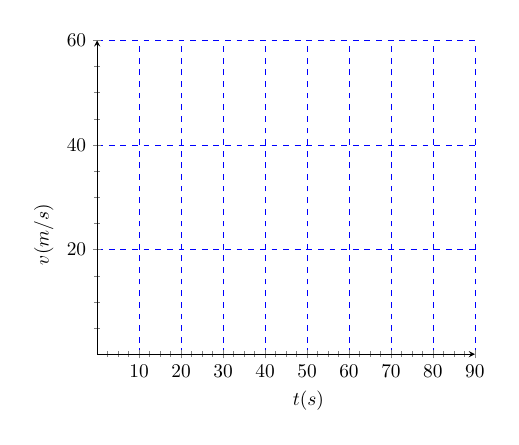
\begin{tikzpicture}[scale=0.7]
                \centering
                \begin{axis}
                    [axis lines = left,
                    axis x line=center,
                    axis y line=center,
                    mark=circle,
% xtick={-5,-4,...,5},
% ytick={-5,-4,...,5},
                    xlabel={$t(s)$},
                    ylabel={$v(m/s)$},
                    ylabel near ticks,
                    xlabel near ticks,
                    xlabel style={below right},
                    ylabel style={above left},
                    ymax=60,
                    ymin=0,
                    xmax=90,
                    xmin=0,
                    xtick={0,10,20,30,40,50,60,70,80,90},
                    ymajorgrids=true,
                    xmajorgrids=true,
                    minor tick num=3,
                    grid style={dashed, blue},
                    ]
                \end{axis}
        \end{tikzpicture}
        \caption{\textbf{Sistema de referencia}. Se representa la velocidad frente al tiempo.}
        \label{fig:reference_system}
    \end{figure}
\end{minipage}
\hfill
\begin{minipage}{0.45\textwidth}
    Decimos que un objeto está en movimiento cuando su posición cambia con respecto a un sistema de referencia a lo largo del tiempo.

    Si su posición no cambia, decimos que el objeto está en \textbf{reposo}.

    El movimiento es relativo, es decir, depende del punto de referencia, y por ello, para su estudio, es necesario establecer un sistema de referencia.

    En Física, el sistema de referencia será un sistema de coordenadas cartesianas \( x\ ,\ y \).
\end{minipage}

\vspace*{6pt}
\begin{definition}[Sistema de Referencia]
         Es un sistema que nos permite fijar la posición de un objeto y estudiar su evolución a lo largo del tiempo.
\end{definition}

\section{Magnitudes que describen el movimiento}

Para determinar el movimiento, necesitamos conocer las siguientes magnitudes:

\begin{enumerate}[label=\numberballmDarkTeal]
        \item \textbf{Posición}.
        Nos indica la ubicación exacta del objeto.
        La posición se suele representar mediante la letra \( x \), y su unidad en el SI es el metro (\( \unit{\metre} \)).

        \item \textbf{Desplazamiento}.
        Es la diferencia entre la posición final y la posición inicial del movimiento.
        El desplazamiento se representará como \( \Delta x \):

        \vspace*{20pt}
        \begin{centeredequation}
            \eqnmarkbox[blue]{displacement}{\Delta x}
            =
            \eqnmarkbox[red]{finalpos}{x_f}
            -
            \eqnmarkbox[mygreen]{initialpos}{x_i}
        \end{centeredequation}
        \vspace{25pt}
        \annotate[yshift=1em]{left}{displacement}{Desplazamiento}
        \annotate[yshift=1em]{}{finalpos}{Posición final}
        \annotate[yshift=-2em]{below,left}{initialpos}{Posición inicial}

        Matemáticamente, el símbolo \( \Delta \) indica la diferencia entre los valores final e inicial.

        Si este símbolo precede a una magnitud, significa el valor final menos el valor inicial de dicha magnitud.

        Para la posición, tendremos \( \Delta x = x_f - x_i \), para el tiempo \( \Delta t = t_f - t_i \), y para la velocidad \( \Delta v = v_f - v_i \).

        \item Su unidad también será el metro.

        \begin{remark}
            Aquí es importante señalar que el desplazamiento puede ser \textbf{negativo}.
            Esto ocurre cuando el objeto en movimiento se desplaza en sentido contrario.
        \end{remark}

        \item \textbf{Trayectoria}.
        Es el camino seguido durante el movimiento.

        \item \textbf{Distancia recorrida}.
        Es la longitud de la trayectoria.
        Su unidad también será el metro.
\end{enumerate}

El movimiento puede clasificarse según su trayectoria.
Así, tendremos:
\begin{enumerate}[label=\letraminuscula]
        \item \negsubro{Rectilíneo}.
        La trayectoria es una línea recta.
        En este tipo de movimiento, el desplazamiento coincide con la distancia recorrida.
        \item \negsubro{Circular}.
        La trayectoria es circular.
        \item \negsubro{Curvilíneo}.
        La trayectoria describe curvas.
\end{enumerate}

\begin{exercise}
    En tu cuaderno, identifica si la trayectoria de cada uno de los siguientes movimientos es recta (rectilínea) o curva (circular).
    \begin{enumerate}[label=\letraminuscula]
        \item una pelota que cae desde una altura
        \item una piedra atada a una cuerda y girada en círculos
        \item el movimiento de la manecilla de los segundos de un reloj
        \item un velocista que corre \qty{100}{\metre} en una pista recta
    \end{enumerate}
%    Página 135, Ejericio 11
    \begin{solu}
        \textbf{\textcolor{purple}{Ejercicio:}} En tu cuaderno, identifica si la trayectoria de cada uno de los siguientes movimientos es recta (rectilínea) o curva (circular).
        \begin{enumerate}[label=\letraminuscula]
            \item una pelota que cae desde una altura
            \item una piedra atada a una cuerda y girada en círculos
            \item el movimiento de la manecilla de los segundos de un reloj
            \item un velocista que corre \qty{100}{\metre} en una pista recta
        \end{enumerate}

        \vspace{0.3cm}

        \begin{enumerate}[label=\letraminuscula]
            \item \textcolor{blue}{Rectilínea (línea recta)} - Una pelota que cae se mueve verticalmente hacia abajo en una trayectoria recta debido a la gravedad.
            \item \textcolor{blue}{Circular} - Una piedra atada a una cuerda y girada traza una trayectoria circular alrededor del punto central.
            \item \textcolor{blue}{Circular} - La manecilla de los segundos de un reloj se mueve en una trayectoria circular alrededor de la esfera del reloj.
            \item \textcolor{blue}{Rectilínea (línea recta)} - Un velocista que corre 100 m en una pista recta sigue una trayectoria lineal.
        \end{enumerate}
    \end{solu}
\end{exercise}

\begin{exercise}
    Imagina que das una vuelta completa a una rotonda circular y regresas a tu posición de partida. ¿Cuál es tu desplazamiento total?
    \begin{solu}
        \textbf{\textcolor{purple}{Ejercicio:}} Imagina que das una vuelta completa a una rotonda circular y regresas a tu posición de partida. ¿Cuál es tu desplazamiento total?

        \vspace{0.3cm}

        \textcolor{red}{Concepto clave:} El desplazamiento es una magnitud vectorial que mide el cambio de posición desde el punto inicial hasta el punto final.

        \textcolor{blue}{Datos:}
        \begin{itemize}
            \item Posición inicial = Posición final (regresas al lugar donde empezaste)
        \end{itemize}

        \textcolor{blue}{Análisis:}

        El desplazamiento se define como:
        \[
            \vec{\Delta x} = \vec{x}_{\text{final}} - \vec{x}_{\text{inicial}}
        \]

        Dado que regresas al punto de partida:
        \[
            \vec{x}_{\text{final}} = \vec{x}_{\text{inicial}}
        \]

        Por lo tanto:
        \[
            \vec{\Delta x} = \vec{x}_{\text{inicial}} - \vec{x}_{\text{inicial}} = \vec{0}
        \]

        \textcolor{red}{Respuesta:} El desplazamiento es \textbf{cero} (\qty{0}{\m}), aunque hayas recorrido una cierta distancia alrededor de la rotonda. Esto demuestra la diferencia entre distancia (longitud total del camino recorrido) y desplazamiento (cambio de posición en línea recta).
    \end{solu}
\end{exercise}

\begin{exercise}
    Si das toda la vuelta a una rotonda y regresas al punto de partida, ¿cuál es tu desplazamiento?
    \begin{solu}
        El desplazamiento es la distancia en línea recta entre el inicio y el final.
        \begin{itemize}
            \item \textbf{Posición inicial ($x_i$):} Punto A.
            \item \textbf{Posición final ($x_f$):} Punto A.
            \item \textbf{Cálculo:} $\Delta x = x_f - x_i = A - A = \mathbf{0}$.
        \end{itemize}
        El desplazamiento es \textcolor{red}{\qty{0}{\m}}. Observa que la \textit{distancia recorrida} es el perímetro de la rotonda, pero el desplazamiento es cero.
    \end{solu}
\end{exercise}


\section{Velocidad}

La velocidad nos da una medida de la rapidez con la que se mueve un objeto.
Tenemos dos tipos de velocidad:

\begin{enumerate}[label=\numberballmDarkTeal]
        \item \textbf{Velocidad instantánea}.
        Es la velocidad que tiene un objeto en un instante dado.
        Podemos verla en el velocímetro de un coche, ya que la velocidad cambia constantemente.

        \item \textbf{Velocidad media}.
        Esta es la medida de velocidad que utilizaremos en este curso y la representaremos con la letra \( v \).
        \begin{centeredequation}
            v = \dfrac{\text{Desplazamiento}}{\text{Tiempo transcurrido}} = \dfrac{\Delta x}{\Delta t}
        \end{centeredequation}

        \item Si expresamos esto en términos de la posición inicial y final, tenemos:
        \begin{centeredequation}
            v = \dfrac{x_f - x_i}{t_f - t_i}
        \end{centeredequation}
        \begin{itemize}
            \item \( x_i \) es la posición inicial.
            \item \( t_i \) es el tiempo medido en la posición inicial.
            \item \( x_f \) es la posición final.
            \item \( t_f \) es el tiempo medido en la posición final.
        \end{itemize}
\end{enumerate}

Las unidades del SI para la velocidad son: \unit{\mps}


\section{Aceleración}

La aceleración nos indica cómo cambia la velocidad con el tiempo.
Al igual que la velocidad, tenemos dos tipos de aceleración:

\begin{enumerate}[label=\numberballmDarkTeal]
        \item \textbf{Aceleración instantánea}.
        Es la aceleración en un instante dado.

        \item \textbf{Aceleración media}.
        Es la aceleración a lo largo de un periodo de tiempo.
        Esta es la que utilizaremos en este tema.
        La fórmula se expresa como:
        \begin{centeredequation}
            a = \dfrac{\text{Cambio de velocidad}}{\text{Tiempo transcurrido}} = \dfrac{\Delta v}{\Delta t}
        \end{centeredequation}

        \item Si expresamos esto en términos de la velocidad inicial y final, tenemos:
        \begin{centeredequation}
            a = \dfrac{v_f - v_i}{t_f - t_i}
        \end{centeredequation}
        \begin{itemize}
            \item \( v_i \) es la velocidad inicial.
            \item \( t_i \) es el tiempo medido en la velocidad inicial.
            \item \( v_f \) es la velocidad final.
            \item \( t_f \) es el tiempo medido en la velocidad final.
        \end{itemize}
\end{enumerate}

Las unidades del SI para la aceleración son: \unit{\mpss}


\section{Movimiento Rectilíneo}

Los movimientos rectilíneos son aquellos que tienen una \textbf{trayectoria en línea recta}.
Estos movimientos son muy interesantes porque, en estos casos, \textbf{el desplazamiento coincide con la distancia recorrida}.

Las ecuaciones descritas anteriormente para la velocidad y la aceleración pueden escribirse como:
\begin{centeredequation}
    v = \dfrac{\Delta x}{\Delta t} \longrightarrow v = \dfrac{x_f - x_i}{t_f - t_i}
\end{centeredequation}
\begin{centeredequation}
    a = \dfrac{\Delta v}{\Delta t} \longrightarrow a = \dfrac{v_f - v_i}{t_f - t_i}
\end{centeredequation}
A veces estas expresiones pueden simplificarse porque:
\begin{itemize}
    \item Generalmente, tomamos \( t_i = 0 \), por lo que este término puede eliminarse.
    Podemos elegir el instante inicial.
    \item Como solo queda un término de tiempo, \( t_f \) puede simplificarse simplemente como \( t \).
    \item Lo mismo se aplica a \( x_i \), aunque es menos habitual.
    Si fijamos la posición inicial \( x_i = 0 \), puede eliminarse, y la posición final \( x_f \) puede llamarse simplemente \( x \).
    \item La misma simplificación puede aplicarse también a \( v_i \).
\end{itemize}
Tras estas simplificaciones, las ecuaciones quedan:
\begin{centeredequation}
    v = \dfrac{x}{t}
\end{centeredequation}
\begin{centeredequation}
    a = \dfrac{v}{t}
\end{centeredequation}
\begin{remark}
    Aunque podamos simplificar las expresiones, es importante leer con atención el enunciado del problema para comprobar si la simplificación está permitida.
\end{remark}

\subsection{Movimiento Rectilíneo Uniforme (MRU)}

Este es un caso particular de movimiento rectilíneo con las siguientes condiciones:
\begin{itemize}
    \item Su trayectoria es una línea recta.
    \item Su velocidad no cambia durante el movimiento. Por lo tanto:
    \begin{itemize}
        \item \( v_f = v_i \)
        \item \( \Delta v = 0 \)
    \end{itemize}
    \item Dado que la velocidad no cambia, la aceleración es cero, es decir, \( a = \qty{0}{\mpss} \)

    \begin{theorem}[]
        La velocidad viene dada por: $v = \dfrac{x_f - x_i}{t_f-t_i}$. Aplicando las simplificaciones anteriores: \(  v = \dfrac{x}{t}  \)

%        To find the final position:
%        \begin{centeredequation}
%            x_f = x_i + v\cdot (t_f-t_i)
%        \end{centeredequation}
%        If \( t_i = 0 \):
%        \begin{centeredequation}
%            x_f = x_i + v\cdot t
%        \end{centeredequation}
%        If also \( x_i = 0 \):
%        \begin{centeredequation}
%            x = v\cdot t
%        \end{centeredequation}
%        To find \( t_f \):
%        \begin{centeredequation}
%            t_f = t_i + \dfrac{x_f-x_i}{v}
%        \end{centeredequation}
%        If \( t_i = 0 \):
%        \begin{centeredequation}
%            t = \dfrac{x_f-x_i}{v}
%        \end{centeredequation}
%        If \( x_i = 0 \):
%        \begin{centeredequation}
%            t = \dfrac{x}{v}
%        \end{centeredequation}
    \end{theorem}
\end{itemize}


%    Página 135, Ejericio 12

\begin{exercise}
    El Sol se encuentra a una distancia media de \qty{1.5e8}{\kilo\m} de la Tierra, y la velocidad de la luz en el vacío es \qty{3e8}{\mps}. Suponiendo que la luz viaja a velocidad constante (movimiento rectilíneo uniforme), calcula cuánto tiempo tarda la luz del Sol en llegar a la Tierra.

    \begin{solu}
        \textbf{\textcolor{purple}{Ejercicio:}} El Sol se encuentra a una distancia media de \qty{1.5e8}{\kilo\m} de la Tierra, y la velocidad de la luz en el vacío es \qty{3e8}{\mps}. Suponiendo que la luz viaja a velocidad constante (movimiento rectilíneo uniforme), calcula cuánto tiempo tarda la luz del Sol en llegar a la Tierra.

        \vspace{0.3cm}

        \textcolor{blue}{Datos:}
        \begin{itemize}
            \item Distancia del Sol a la Tierra: $d = \qty{1.5e8}{\kilo\m}$
            \item Velocidad de la luz: $v = \qty{3e8}{\mps}$
            \item Tipo de movimiento: Movimiento rectilíneo uniforme (velocidad constante)
        \end{itemize}

        \textcolor{blue}{Paso 1: Convertir todas las unidades al SI (metros y segundos)}
        \[
            d = 1.5 \times 10^8 \text{ km} \times \frac{1000 \text{ m}}{1 \text{ km}} = \textcolor{red}{1.5 \times 10^{11} \text{ m}}
        \]

        \textcolor{blue}{Paso 2: Aplicar la fórmula del movimiento uniforme}

        Para el movimiento rectilíneo uniforme, la relación entre distancia, velocidad y tiempo es:
        \[
            \boxed{d = v \cdot t}
        \]

        \textcolor{blue}{Paso 3: Despejar el tiempo}

        Reordenando la ecuación:
        \[
            t = \frac{d}{v}
        \]

        \textcolor{blue}{Paso 4: Sustituir valores y calcular}
        \[
            t = \frac{1.5 \times 10^{11} \text{ m}}{3 \times 10^8 \text{ m/s}} = \frac{1.5}{3} \times 10^{11-8} \text{ s} = 0.5 \times 10^3 \text{ s} = \textcolor{red}{500 \text{ s}}
        \]

        \textcolor{blue}{Paso 5: Convertir a minutos (opcional)}
        \[
            t = 500 \text{ s} \times \frac{1 \text{ min}}{60 \text{ s}} = \textcolor{red}{8.33 \text{ min}} \approx 8 \text{ min } 20 \text{ s}
        \]

        \textcolor{red}{Respuesta:} La luz tarda aproximadamente \textbf{500 segundos} (u \textbf{8 minutos y 20 segundos}) en viajar desde el Sol hasta la Tierra.
    \end{solu}
\end{exercise}


\begin{exercise}
    Durante una clase de Educación Física, estás cronometrando cuánto tardan los estudiantes en correr \qty{100}{\m}.
    \begin{enumerate}[label=\letraminuscula]
        \item Si una de tus compañeras completa los \qty{100}{\m} en \qty{15}{\s}, ¿cuál es su velocidad media?
        \item De media, ¿cuántos metros recorre cada segundo?
    \end{enumerate}
    \begin{solu}
        \textbf{\textcolor{purple}{Ejercicio:}} Durante una clase de Educación Física, estás cronometrando cuánto tardan los estudiantes en correr \qty{100}{\m}.
        \begin{enumerate}[label=\letraminuscula]
            \item Si una de tus compañeras completa los \qty{100}{\m} en \qty{15}{\s}, ¿cuál es su velocidad media?
            \item De media, ¿cuántos metros recorre cada segundo?
        \end{enumerate}

        \vspace{0.3cm}

        \textcolor{blue}{Datos:}
        \begin{itemize}
            \item Distancia: $d = \qty{100}{\m}$
            \item Tiempo: $t = \qty{15}{\s}$
        \end{itemize}

        \textbf{\textcolor{blue}{Apartado a) Calcular la velocidad media}}

        \textcolor{blue}{Paso 1: Aplicar la fórmula de la velocidad media}

        La velocidad media se define como:
        \[
            \boxed{v_{\text{media}} = \frac{d}{t}}
        \]

        \textcolor{blue}{Paso 2: Sustituir valores y calcular}
        \[
            v_{\text{media}} = \frac{100 \text{ m}}{15 \text{ s}} = \textcolor{red}{6.67 \text{ m/s}}
        \]

        \textcolor{red}{Respuesta a):} Su velocidad media es \textbf{\qty{6.67}{\mps}}.

        \vspace{0.5cm}

        \textbf{\textcolor{blue}{Apartado b) Metros por segundo}}

        \textcolor{blue}{Análisis:} La pregunta plantea «cuántos metros recorre por segundo», que es exactamente la definición de la rapidez en m/s.

        \textcolor{red}{Respuesta b):} Recorre una media de \textbf{6,67 metros por segundo}. Este es el mismo valor que la velocidad calculada en el apartado a), ya que la velocidad se mide en metros por segundo (m/s).
    \end{solu}
\end{exercise}



\begin{exercise}
    Durante un viaje familiar en coche, tu coche circula por una autovía recta a una velocidad media de \qty{90}{\kmph} durante \qty{15}{min}.
    \begin{enumerate}[label=\letraminuscula]
        \item Calcula la distancia recorrida en metros durante este periodo de tiempo.
        \item ¿Puedes estar seguro de que la velocidad del coche fue exactamente \qty{90}{\kmph} en todo momento durante el trayecto?
    \end{enumerate}
    \begin{solu}
        \textbf{\textcolor{purple}{Ejercicio:}} Durante un viaje familiar en coche, tu coche circula por una autovía recta a una velocidad media de \qty{90}{\kmph} durante \qty{15}{min}.
        \begin{enumerate}[label=\letraminuscula]
            \item Calcula la distancia recorrida en metros durante este periodo de tiempo.
            \item ¿Puedes estar seguro de que la velocidad del coche fue exactamente \qty{90}{\kmph} en todo momento durante el trayecto?
        \end{enumerate}

        \vspace{0.3cm}

        \textcolor{blue}{Datos:}
        \begin{itemize}
            \item Velocidad media: $v_{\text{media}} = \qty{90}{\kmph}$
            \item Tiempo: $t = \qty{15}{min}$
        \end{itemize}

        \textbf{\textcolor{blue}{Apartado a) Calcular la distancia en metros}}

        \textcolor{blue}{Paso 1: Convertir las unidades al SI}

        Convertir la velocidad de km/h a m/s:
        \[
            v = 90 \frac{\text{km}}{\text{h}} \times \frac{1000 \text{ m}}{1 \text{ km}} \times \frac{1 \text{ h}}{3600 \text{ s}} = 90 \times \frac{1000}{3600} = \textcolor{red}{25 \text{ m/s}}
        \]

        Convertir el tiempo de minutos a segundos:
        \[
            t = 15 \text{ min} \times \frac{60 \text{ s}}{1 \text{ min}} = \textcolor{red}{900 \text{ s}}
        \]

        \textcolor{blue}{Paso 2: Aplicar la fórmula de la distancia}
        \[
            \boxed{d = v \cdot t}
        \]

        \textcolor{blue}{Paso 3: Calcular la distancia}
        \[
            d = 25 \text{ m/s} \times 900 \text{ s} = \textcolor{red}{22\,500 \text{ m}}
        \]

        \textcolor{red}{Respuesta a):} El coche recorrió \textbf{\qty{22500}{\m}} (o 22,5 km) durante esos 15 minutos.

        \vspace{0.5cm}

        \textbf{\textcolor{blue}{Apartado b) ¿Fue la velocidad constante?}}

        \textcolor{blue}{Análisis:} El enunciado indica que 90 km/h es la velocidad \textit{media}, no la velocidad instantánea.

        \textcolor{red}{Respuesta b):} \textbf{No}, no podemos estar seguros de que la velocidad fuera exactamente 90 km/h en todo momento. El valor de 90 km/h es la \textit{velocidad media} durante el intervalo de 15 minutos. Durante el trayecto, el coche pudo haber circulado más rápido o más despacio en distintos momentos (por ejemplo, acelerando para adelantar, reduciendo la velocidad en las curvas, etc.), siempre que la media a lo largo de todo el periodo de tiempo sea igual a 90 km/h.
    \end{solu}
\end{exercise}


\begin{exercise}
    Un coche que circula por una autovía recta lleva viajando durante \qty{30}{min} a una velocidad media de \qty{100}{\kmph}. ¿Qué distancia, en metros, ha recorrido el coche durante este tiempo?
    \begin{solu}
        \textbf{\textcolor{purple}{Ejercicio:}} Un coche que circula por una autovía recta lleva viajando durante \qty{30}{min} a una velocidad media de \qty{100}{\kmph}. ¿Qué distancia, en metros, ha recorrido el coche durante este tiempo?

        \vspace{0.3cm}

        \textcolor{blue}{Datos:}
        \begin{itemize}
            \item Velocidad media: $v_{\text{media}} = \qty{100}{\kmph}$
            \item Tiempo: $t = \qty{30}{min}$
        \end{itemize}

        \textcolor{blue}{Paso 1: Convertir las unidades al SI}

        Convertir la velocidad de km/h a m/s:
        \[
            v = 100 \frac{\text{km}}{\text{h}} \times \frac{1000 \text{ m}}{1 \text{ km}} \times \frac{1 \text{ h}}{3600 \text{ s}} = 100 \times \frac{1000}{3600} = \textcolor{red}{27.78 \text{ m/s}}
        \]

        Convertir el tiempo de minutos a segundos:
        \[
            t = 30 \text{ min} \times \frac{60 \text{ s}}{1 \text{ min}} = \textcolor{red}{1800 \text{ s}}
        \]

        \textcolor{blue}{Paso 2: Aplicar la fórmula de la distancia para el movimiento uniforme}
        \[
            \boxed{d = v \cdot t}
        \]

        \textcolor{blue}{Paso 3: Sustituir valores y calcular}
        \[
            d = 27.78 \text{ m/s} \times 1800 \text{ s} = \textcolor{red}{50\,000 \text{ m}}
        \]

        \textcolor{red}{Respuesta:} El coche ha recorrido \textbf{\qty{50000}{\m}} (o 50 km) durante los 30 minutos.
    \end{solu}
\end{exercise}


\begin{exercise}
    Un coche se mueve por una carretera recta, y su velocidad cambia de la siguiente manera: Tras \qty{1}{\s}, su velocidad es \qty{2}{\mps}. Tras \qty{2}{\s} desde el inicio, su velocidad es \qty{4}{\mps}. Tras \qty{3}{\s}, su velocidad es \qty{6}{\mps}.

    \begin{enumerate}[label=\letraminuscula]
        \item ¿En cuánto cambia la velocidad del coche durante cada segundo?
        \item ¿Cuál es la aceleración de este vehículo?
    \end{enumerate}
    \begin{solu}
        \textbf{\textcolor{purple}{Ejercicio:}} Un coche se mueve por una carretera recta, y su velocidad cambia de la siguiente manera: Tras \qty{1}{\s}, su velocidad es \qty{2}{\mps}. Tras \qty{2}{\s} desde el inicio, su velocidad es \qty{4}{\mps}. Tras \qty{3}{\s}, su velocidad es \qty{6}{\mps}.
        \begin{enumerate}[label=\letraminuscula]
            \item ¿En cuánto cambia la velocidad del coche durante cada segundo?
            \item ¿Cuál es la aceleración de este vehículo?
        \end{enumerate}

        \vspace{0.3cm}

        \textcolor{blue}{Datos:}
        \begin{itemize}
            \item En $t_1 = 1$ s: $v_1 = \qty{2}{\mps}$
            \item En $t_2 = 2$ s: $v_2 = \qty{4}{\mps}$
            \item En $t_3 = 3$ s: $v_3 = \qty{6}{\mps}$
        \end{itemize}

        \textbf{\textcolor{blue}{Apartado a) Cambio de velocidad por segundo}}

        \textcolor{blue}{Paso 1: Calcular los cambios de velocidad}

        Cambio durante el primer segundo (de $t=0$ a $t=1$ s):
        \[
            \Delta v_1 = v_1 - v_0 = 2 - 0 = \textcolor{red}{2 \text{ m/s}}
        \]

        Cambio durante el segundo segundo (de $t=1$ a $t=2$ s):
        \[
            \Delta v_2 = v_2 - v_1 = 4 - 2 = \textcolor{red}{2 \text{ m/s}}
        \]

        Cambio durante el tercer segundo (de $t=2$ a $t=3$ s):
        \[
            \Delta v_3 = v_3 - v_2 = 6 - 4 = \textcolor{red}{2 \text{ m/s}}
        \]

        \textcolor{red}{Respuesta a):} La velocidad del coche aumenta en \textbf{\qty{2}{\mps}} durante cada segundo.

        \vspace{0.5cm}

        \textbf{\textcolor{blue}{Apartado b) Calcular la aceleración}}

        \textcolor{blue}{Paso 2: Aplicar la fórmula de la aceleración}

        La aceleración se define como la tasa de cambio de la velocidad:
        \[
            \boxed{a = \frac{\Delta v}{\Delta t}}
        \]

        Dado que la velocidad cambia en 2 m/s cada 1 segundo:
        \[
            a = \frac{2 \text{ m/s}}{1 \text{ s}} = \textcolor{red}{2 \text{ m/s}^2}
        \]

        \textcolor{blue}{Cálculo alternativo usando dos puntos cualesquiera:}
        \[
            a = \frac{v_3 - v_1}{t_3 - t_1} = \frac{6 - 2}{3 - 1} = \frac{4}{2} = \textcolor{red}{2 \text{ m/s}^2}
        \]

        \textcolor{red}{Respuesta b):} La aceleración del vehículo es \textbf{\qty{2}{\metre\per\second\squared}}.

        \textcolor{blue}{Nota:} Dado que la aceleración es constante y positiva, se trata de un movimiento uniformemente acelerado.
    \end{solu}
\end{exercise}

\begin{exercise}
    Un ciclista sale de Almansa por el carril bici a una velocidad de \qty{8}{\mps}.
    Si tarda \qty{100}{\min} en llegar a su destino:
    \begin{enumerate}[label=\letraminuscula]
    \item ¿Qué distancia ha recorrido?
    \item Sabiendo que Bonete está a \qty{32}{\km}, ¿cuánto tardaría en llegar?
    \end{enumerate}
\end{exercise}

\subsubsection{Gráficas del Movimiento Rectilíneo Uniforme (MRU)}
En física, es muy habitual elaborar gráficas y, a partir de ellas, identificar el tipo de movimiento. Para el MRU, tendremos los siguientes casos.
\begin{figure}[H]
    \centering
    % First subfigure
    \begin{subfigure}[b]{0.45\textwidth}
        \centering
        \begin{tikzpicture}[scale=0.85]
            \begin{axis}
                [
                ylabel={$x$ (\unit{\m})},
                xlabel={$t$ (\unit{\s})},
                axis lines=middle,
                enlargelimits=true,
                xmin=0, xmax=10,
                ymin=0, ymax=10,
                domain=0:8,
                samples=100,
                legend pos=outer north east,
                legend style={draw=none},
                xticklabels={},
                yticklabels={}
                ]
                \addplot[line width=1.5pt, red] {3 + 0.5*x};
            \end{axis}
        \end{tikzpicture}
        \caption{Posición frente a Tiempo. Moviéndose en sentido positivo.}
    \end{subfigure}
    \hfill
    % Second subfigure
    \begin{subfigure}[b]{0.45\textwidth}
        \centering
        \begin{tikzpicture}[scale=0.85]
            \begin{axis}
                [
                ylabel={$x$ (\unit{\m})},
                xlabel={$t$ (\unit{\s})},
                axis lines=middle,
                enlargelimits=true,
                xmin=0, xmax=10,
                ymin=0, ymax=10,
                domain=0:8,
                samples=100,
                legend pos=outer north east,
                legend style={draw=none},
                xticklabels={},
                yticklabels={}
                ]
                \addplot[line width=1.5pt, red] {8 - 0.5*x};
            \end{axis}
        \end{tikzpicture}
        \caption{Posición frente a Tiempo. Moviéndose en sentido contrario.}
    \end{subfigure}
\end{figure}

\begin{figure}[H]
    \centering
    % First subfigure
    \begin{subfigure}[b]{0.45\textwidth}
        \centering
        \begin{tikzpicture}[scale=0.85]
            \begin{axis}
                [
                ylabel={$v$ (\unit{\mps})},
                xlabel={$t$ (\unit{\s})},
                axis lines=middle,
                enlargelimits=true,
                xmin=0, xmax=10,
                ymin=0, ymax=10,
                domain=0:8,
                samples=100,
                legend pos=outer north east,
                legend style={draw=none},
                xticklabels={},
                yticklabels={}
                ]
                \addplot[line width=1.5pt, red] {5};
            \end{axis}
        \end{tikzpicture}
        \caption{Velocidad frente a Tiempo. Moviéndose en sentido positivo.}
    \end{subfigure}
    \hfill
    % Second subfigure
    \begin{subfigure}[b]{0.45\textwidth}
        \centering
        \begin{tikzpicture}[scale=0.85]
            \begin{axis}
                [
                ylabel={$a$ (\unit{\mpss})},
                xlabel={$t$ (\unit{\s})},
                axis lines=middle,
                enlargelimits=true,
                xmin=0, xmax=10,
                ymin=-1, ymax=10,
                domain=0:8,
                samples=100,
                legend style={draw=none},
                xticklabels={},
                yticklabels={}
                ]
                \addplot[line width=2pt, red] {0};
            \end{axis}
        \end{tikzpicture}
        \caption{Aceleración frente a Tiempo.}
    \end{subfigure}
\end{figure}
%\begin{remark}
%    If the motion is in the opposite direction, the velocity vs time graph would look like:
%    \begin{figure}[H]
%        \centering
%        \begin{tikzpicture}[scale=0.85]
%            \begin{axis}
%                [
%                ylabel={$v$ (\unit{\mps})},
%                xlabel={$t$ (\unit{\s})},
%                axis lines=middle,
%                enlargelimits=true,
%                xmin=-10, xmax=2,
%                ymin=0, ymax=10,
%                domain=-10:2,
%                samples=100,
%                legend pos=outer north east,
%                legend style={draw=none},
%                xticklabels={},
%                yticklabels={}
%                ]
%                \addplot[line width=1.5pt, red] {-5};
%            \end{axis}
%        \end{tikzpicture}
%        \caption{Velocity vs Time. Moving in the opposite direction.}
%    \end{figure}
%\end{remark}


\subsection{Movimiento Rectilíneo Uniformemente Acelerado (MRUA)}

Este es otro caso particular de movimiento rectilíneo que cumple las siguientes condiciones:
\begin{itemize}
    \item La trayectoria también es una línea recta.
    \item Ahora, la velocidad cambia durante el movimiento.
    \begin{itemize}
        \item \( v_f \neq v_i \)
        \item \( \Delta v \neq  0 \)
    \end{itemize}
    \item Dado que la velocidad cambia, la aceleración ahora es distinta de cero (\( a \neq 0 \)) pero constante, lo que significa que la aceleración no varía.
\end{itemize}

Las ecuaciones de este movimiento son las siguientes:
\begin{itemize}
    \item Para la aceleración tenemos:
    \begin{centeredequation}
        a = \dfrac{v_f - v_i}{t_f - t_i} \label{eq:aceleracion_general}
    \end{centeredequation}
    Si aplicamos las simplificaciones \( v_i = 0 \) y \( t_i = 0 \), obtenemos:
    \begin{centeredequation}
        a = \dfrac{v}{t}
    \end{centeredequation}
    \item La ecuación de la posición es:
    \begin{centeredequation}
        x_f = x_i + v_i\cdot (t_f - t_i) + \frac{1}{2} \cdot a \cdot (t_f - t_i)^2 \label{eq:posición_general}
    \end{centeredequation}
    Si simplificamos suponiendo que el instante inicial es \( t_i = 0 \), la ecuación queda:
    \begin{centeredequation}
        x_f = x_i + v_i \cdot t + \frac{1}{2} \cdot a \cdot t^2
    \end{centeredequation}
    Si además suponemos que la posición inicial es cero (\( x_i = 0 \)), esta expresión se simplifica aún más:
    \begin{centeredequation}
        x = v_i \cdot t + \frac{1}{2} \cdot a \cdot t^2
    \end{centeredequation}
    Como podemos observar, en esta ecuación \( v_f \) nunca aparece, lo que significa que la posición final no depende de la velocidad final, pero sí depende de la velocidad inicial, ya que esta aparece en la fórmula.
    \item Debido a la complejidad de despejar el tiempo en este tipo de movimiento, la expresión no se estudiará en este curso.
\end{itemize}


\begin{exercise}
    Has ido a esquiar con tus compañeros de clase y decides bajar por una pista. Partiendo del reposo, aceleras hasta \qty{10}{\mps} en \qty{5}{\s}. ¿Cuál fue tu aceleración media?
    \begin{solu}
        \textbf{\textcolor{purple}{Ejercicio:}} Has ido a esquiar con tus compañeros de clase y decides bajar por una pista. Partiendo del reposo, aceleras hasta \qty{10}{\mps} en \qty{5}{\s}. ¿Cuál fue tu aceleración media?

        \vspace{0.3cm}

        \textcolor{blue}{Datos:}
        \begin{itemize}
            \item Velocidad inicial: $v_0 = \qty{0}{\mps}$ (partiendo del reposo)
            \item Velocidad final: $v_f = \qty{10}{\mps}$
            \item Intervalo de tiempo: $\Delta t = \qty{5}{\s}$
        \end{itemize}

        \textcolor{blue}{Paso 1: Aplicar la fórmula de la aceleración}

        La aceleración se define como el cambio de velocidad dividido por el intervalo de tiempo:
        \[
            \boxed{a = \frac{\Delta v}{\Delta t} = \frac{v_f - v_0}{\Delta t}}
        \]

        \textcolor{blue}{Paso 2: Calcular el cambio de velocidad}
        \[
            \Delta v = v_f - v_0 = 10 - 0 = \textcolor{red}{10 \text{ m/s}}
        \]

        \textcolor{blue}{Paso 3: Calcular la aceleración}
        \[
            a = \frac{10 \text{ m/s}}{5 \text{ s}} = \textcolor{red}{2 \text{ m/s}^2}
        \]

        \textcolor{red}{Respuesta:} Tu aceleración media al bajar por la pista fue \textbf{\qty{2}{\metre\per\second\squared}}.

        \textcolor{blue}{Interpretación física:} Esto significa que tu velocidad aumentó 2 m/s cada segundo durante el descenso.
    \end{solu}
\end{exercise}


\begin{exercise}
    Un vehículo acelera desde el reposo hasta \qty{100}{\kmph} en \qty{8}{\s}. Calcula su aceleración media, dando tu respuesta en \unit{\mpss}.
    \begin{solu}
        \textbf{\textcolor{purple}{Ejercicio:}} Un vehículo acelera desde el reposo hasta \qty{100}{\kmph} en \qty{8}{\s}. Calcula su aceleración media, dando tu respuesta en \unit{\mpss}.

        \vspace{0.3cm}

        \textcolor{blue}{Datos:}
        \begin{itemize}
            \item Velocidad inicial: $v_0 = \qty{0}{\kmph}$ (partiendo del reposo)
            \item Velocidad final: $v_f = \qty{100}{\kmph}$
            \item Intervalo de tiempo: $\Delta t = \qty{8}{\s}$
        \end{itemize}

        \textcolor{blue}{Paso 1: Convertir la velocidad a m/s}

        Velocidad inicial (ya es cero en cualquier unidad):
        \[
            v_0 = 0 \text{ m/s}
        \]

        Velocidad final:
        \[
            v_f = 100 \frac{\text{km}}{\text{h}} \times \frac{1000 \text{ m}}{1 \text{ km}} \times \frac{1 \text{ h}}{3600 \text{ s}} = 100 \times \frac{1000}{3600} = \textcolor{red}{27.78 \text{ m/s}}
        \]

        \textcolor{blue}{Paso 2: Aplicar la fórmula de la aceleración}
        \[
            \boxed{a = \frac{\Delta v}{\Delta t} = \frac{v_f - v_0}{\Delta t}}
        \]

        \textcolor{blue}{Paso 3: Calcular el cambio de velocidad}
        \[
            \Delta v = v_f - v_0 = 27.78 - 0 = \textcolor{red}{27.78 \text{ m/s}}
        \]

        \textcolor{blue}{Paso 4: Calcular la aceleración}
        \[
            a = \frac{27.78 \text{ m/s}}{8 \text{ s}} = \textcolor{red}{3.47 \text{ m/s}^2}
        \]

        \textcolor{red}{Respuesta:} La aceleración media del vehículo es \textbf{\qty{3.47}{\metre\per\second\squared}}.

        \textcolor{blue}{Interpretación física:} La velocidad del vehículo aumenta aproximadamente 3,47 m/s cada segundo durante el periodo de aceleración.
    \end{solu}
\end{exercise}


\begin{exercise}
    Un coche que circula a \qty{30}{\mps} frena durante \qty{5}{\s}, reduciendo su velocidad a \qty{25}{\mps}. Determina su aceleración media durante el frenado.
    \begin{solu}
        \textbf{\textcolor{purple}{Ejercicio:}} Un coche que circula a \qty{30}{\mps} frena durante \qty{5}{\s}, reduciendo su velocidad a \qty{25}{\mps}. Determina su aceleración media durante el frenado.

        \vspace{0.3cm}

        \textcolor{blue}{Datos:}
        \begin{itemize}
            \item Velocidad inicial: $v_0 = \qty{30}{\mps}$
            \item Velocidad final: $v_f = \qty{25}{\mps}$
            \item Intervalo de tiempo: $\Delta t = \qty{5}{\s}$
        \end{itemize}

        \textcolor{blue}{Paso 1: Aplicar la fórmula de la aceleración}
        \[
            \boxed{a = \frac{\Delta v}{\Delta t} = \frac{v_f - v_0}{\Delta t}}
        \]

        \textcolor{blue}{Paso 2: Calcular el cambio de velocidad}
        \[
            \Delta v = v_f - v_0 = 25 - 30 = \textcolor{red}{-5 \text{ m/s}}
        \]

        \textcolor{blue}{Nota:} El cambio de velocidad es negativo porque el coche está frenando.

        \textcolor{blue}{Paso 3: Calcular la aceleración}
        \[
            a = \frac{-5 \text{ m/s}}{5 \text{ s}} = \textcolor{red}{-1 \text{ m/s}^2}
        \]

        \textcolor{red}{Respuesta:} La aceleración media durante el frenado es \textbf{\qty{-1}{\metre\per\second\squared}}.

        \textcolor{blue}{Interpretación física:} El signo negativo indica que se trata de una deceleración (el coche está frenando). El valor absoluto de la aceleración es 1 m/s², lo que significa que la velocidad del coche disminuye 1 m/s cada segundo durante el frenado.
    \end{solu}
\end{exercise}


\begin{exercise}
    Para despegar, un avión Airbus necesita alcanzar una velocidad de \qty{300}{\kmph} en un tiempo de \qty{23.8}{\s}. Calcula:
    \begin{enumerate}[label=\letraminuscula]
    \item ¿Cuál es su aceleración?
    \item ¿Cuál es la longitud mínima de pista necesaria?
    \end{enumerate}
    \begin{solu}
        \textbf{\textcolor{purple}{Ejercicio:}} Para despegar, un avión Airbus necesita alcanzar una velocidad de \qty{300}{\kmph} en un tiempo de \qty{23.8}{\s}. Calcula:
        \begin{enumerate}[label=\letraminuscula]
            \item ¿Cuál es su aceleración?
            \item ¿Cuál es la longitud mínima de pista necesaria?
        \end{enumerate}

        \vspace{0.3cm}

        \textcolor{blue}{Datos:}
        \begin{itemize}
            \item Velocidad inicial: $v_0 = \qty{0}{\kmph}$ (parte del reposo)
            \item Velocidad final: $v_f = \qty{300}{\kmph}$
            \item Tiempo: $t = \qty{23.8}{\s}$
        \end{itemize}

        \textbf{\textcolor{blue}{Apartado a) Calcular la aceleración}}

        \textcolor{blue}{Paso 1: Convertir la velocidad a m/s}
        \[
            v_0 = 0 \text{ m/s}
        \]
        \[
            v_f = 300 \frac{\text{km}}{\text{h}} \times \frac{1000 \text{ m}}{1 \text{ km}} \times \frac{1 \text{ h}}{3600 \text{ s}} = 300 \times \frac{1000}{3600} = \textcolor{red}{83.33 \text{ m/s}}
        \]

        \textcolor{blue}{Paso 2: Aplicar la fórmula de la aceleración}
        \[
            \boxed{a = \frac{v_f - v_0}{t}}
        \]

        \textcolor{blue}{Paso 3: Calcular la aceleración}
        \[
            a = \frac{83.33 - 0}{23.8} = \frac{83.33}{23.8} = \textcolor{red}{3.50 \text{ m/s}^2}
        \]

        \textcolor{red}{Respuesta a):} La aceleración es \textbf{\qty{3.50}{\metre\per\second\squared}}.

        \vspace{0.5cm}

        \textbf{\textcolor{blue}{Apartado b) Calcular la longitud de pista}}

        \textcolor{blue}{Paso 4: Aplicar la ecuación cinemática de la distancia}

        Para un movimiento uniformemente acelerado que parte del reposo, podemos usar:
        \[
            \boxed{d = v_0 \cdot t + \frac{1}{2} a t^2}
        \]

        O alternativamente:
        \[
            \boxed{v_f^2 = v_0^2 + 2ad} \Rightarrow d = \frac{v_f^2 - v_0^2}{2a}
        \]

        \textcolor{blue}{Método 1: Usando $d = v_0 t + \frac{1}{2}at^2$}
        \[
            d = 0 \times 23.8 + \frac{1}{2} \times 3.50 \times (23.8)^2
        \]
        \[
            d = 0 + \frac{1}{2} \times 3.50 \times 566.44 = 1.75 \times 566.44 = \textcolor{red}{991.27 \text{ m}}
        \]

        \textcolor{blue}{Método 2: Usando $d = \frac{v_f^2 - v_0^2}{2a}$}
        \[
            d = \frac{(83.33)^2 - 0^2}{2 \times 3.50} = \frac{6943.89}{7.00} = \textcolor{red}{991.98 \text{ m}}
        \]

        \textcolor{red}{Respuesta b):} La longitud mínima de pista necesaria es de aproximadamente \textbf{\qty{992}{\m}} (o cerca de 1 km).

        \textcolor{blue}{Nota:} Ambos métodos dan esencialmente el mismo resultado; las pequeñas diferencias se deben al redondeo durante los cálculos.
    \end{solu}
\end{exercise}


\begin{exercise}
    Un motorista que circula a \qty{20}{\mps} ve que el semáforo se pone en rojo más adelante. Empieza a frenar y se detiene por completo en \qty{10}{\s}.
    \begin{enumerate}[label=\letraminuscula]
    \item Calcula la aceleración durante el frenado.
    \item Si el semáforo estaba a \qty{90}{\m} del motorista cuando empezó a frenar, ¿consigue detenerse antes de alcanzarlo?
    \end{enumerate}
    \begin{solu}
        \textbf{\textcolor{purple}{Ejercicio:}} Un motorista que circula a \qty{20}{\mps} ve que el semáforo se pone en rojo más adelante. Empieza a frenar y se detiene por completo en \qty{10}{\s}.
        \begin{enumerate}[label=\letraminuscula]
            \item Calcula la aceleración durante el frenado.
            \item Si el semáforo estaba a \qty{90}{\m} del motorista cuando empezó a frenar, ¿consigue detenerse antes de alcanzarlo?
        \end{enumerate}

        \vspace{0.3cm}

        \textcolor{blue}{Datos:}
        \begin{itemize}
            \item Velocidad inicial: $v_0 = \qty{20}{\mps}$
            \item Velocidad final: $v_f = \qty{0}{\mps}$ (se detiene por completo)
            \item Tiempo: $t = \qty{10}{\s}$
            \item Distancia al semáforo: $d_{\text{semáforo}} = \qty{90}{\m}$
        \end{itemize}

        \textbf{\textcolor{blue}{Apartado a) Calcular la aceleración de frenado}}

        \textcolor{blue}{Paso 1: Aplicar la fórmula de la aceleración}
        \[
            \boxed{a = \frac{v_f - v_0}{t}}
        \]

        \textcolor{blue}{Paso 2: Calcular la aceleración}
        \[
            a = \frac{0 - 20}{10} = \frac{-20}{10} = \textcolor{red}{-2 \text{ m/s}^2}
        \]

        \textcolor{red}{Respuesta a):} La aceleración de frenado es \textbf{\qty{-2}{\metre\per\second\squared}}.

        \textcolor{blue}{Nota:} El signo negativo indica deceleración (frenado).

        \vspace{0.5cm}

        \textbf{\textcolor{blue}{Apartado b) ¿Se detiene antes del semáforo?}}

        \textcolor{blue}{Paso 3: Calcular la distancia de frenado}

        Usando la ecuación cinemática:
        \[
            \boxed{d = v_0 \cdot t + \frac{1}{2} a t^2}
        \]

        \textcolor{blue}{Paso 4: Sustituir valores}
        \[
            d_{\text{frenado}} = 20 \times 10 + \frac{1}{2} \times (-2) \times (10)^2
        \]
        \[
            d_{\text{frenado}} = 200 + \frac{1}{2} \times (-2) \times 100
        \]
        \[
            d_{\text{frenado}} = 200 - 100 = \textcolor{red}{100 \text{ m}}
        \]

        \textcolor{blue}{Método alternativo usando: $v_f^2 = v_0^2 + 2ad$}
        \[
            0^2 = 20^2 + 2 \times (-2) \times d
        \]
        \[
            0 = 400 - 4d
        \]
        \[
            d = \frac{400}{4} = \textcolor{red}{100 \text{ m}}
        \]

        \textcolor{blue}{Paso 5: Comparar las distancias}
        \[
            d_{\text{frenado}} = 100 \text{ m} > d_{\text{semáforo}} = 90 \text{ m}
        \]

        \textcolor{red}{Respuesta b):} \textbf{No}, el motorista \textbf{no} consigue detenerse a tiempo. Necesita 100 m para detenerse por completo, pero el semáforo está a solo 90 m. Rebasaría el semáforo en rojo 10 m antes de detenerse.

        \textcolor{blue}{Nota de seguridad:} Esto demuestra la importancia de mantener distancias de seguridad adecuadas y de ser consciente de las distancias de frenado a diferentes velocidades.
    \end{solu}
\end{exercise}



\begin{exercise}
    En un experimento, medimos la posición de un carrito que se mueve en línea recta en distintos instantes. Los datos registrados muestran los tiempos en los que el carrito pasa por diferentes posiciones.
    \begin{table}[H]
        \centering
        \renewcommand{\arraystretch}{1.5}
        \begin{tabular}{Occcc}
            \bottomrule
            \textcolor{ocre}{\textbf{Posición (\unit{\metre})}} & 0 & 3 & 6 & 9 \\
            \hline
            \textcolor{ocre}{\textbf{Tiempo (\unit{\s})}}         & 0 & 1 & 2 & 3 \\
            \toprule
        \end{tabular}
        \label{tab:ejercicio1}
    \end{table}
%    \begin{figure}[H]
%        \centering
%        \includegraphics[scale=0.8]{images/cinematica/ejercicio_40}
%    \end{figure}
    \begin{enumerate}[label=\letraminuscula]
    \item Dibuja la gráfica posición-tiempo.
    \item ¿Qué posición ocupa el carrito respecto al origen tras \qty{3.5}{\s}?
    \item ¿En qué instante el carrito está a \qty{7}{\m} de su posición inicial?
    \end{enumerate}

    \begin{solu}
        \textbf{\textcolor{purple}{Ejercicio:}} En un experimento, medimos la posición de un carrito que se mueve en línea recta en distintos instantes. Los datos registrados muestran los tiempos en los que el carrito pasa por diferentes posiciones.
        \begin{enumerate}[label=\letraminuscula]
            \item Dibuja la gráfica posición-tiempo.
            \item ¿Qué posición ocupa el carrito respecto al origen tras \qty{3.5}{\s}?
            \item ¿En qué instante el carrito está a \qty{7}{\m} de su posición inicial?
        \end{enumerate}

        \vspace{0.3cm}

        \textcolor{red}{Nota:} Dado que los datos reales de la figura no son visibles en el texto, proporcionaré un método de resolución general. Deberías utilizar los valores concretos de la tabla/figura de tu libro.

        \textbf{\textcolor{blue}{Apartado a) Dibujar la gráfica posición-tiempo}}

        \textcolor{blue}{Pasos:}
        \begin{enumerate}
            \item Crea un sistema de coordenadas con el tiempo ($t$) en el eje horizontal y la posición ($x$) en el eje vertical.
            \item Marca los datos de la tabla (tiempo, posición) en la gráfica.
            \item Une los puntos. Si forman una línea recta, el movimiento es uniforme. Si forman una curva, el movimiento es acelerado.
        \end{enumerate}

        \textbf{\textcolor{blue}{Apartado b) Posición en $t = 3,5$ s}}

        \textcolor{blue}{Método:}
        \begin{itemize}
            \item Localiza $t = 3,5$ s en el eje de tiempo
            \item Traza una línea vertical hasta la gráfica
            \item Lee el valor de posición correspondiente en el eje vertical
            \item Si el punto cae entre datos, interpola o usa la ecuación del movimiento
        \end{itemize}

        \textcolor{blue}{Si el movimiento es uniforme:} Usa $x = x_0 + vt$ donde $v$ es la velocidad constante calculada a partir de dos puntos cualesquiera.

        \textcolor{blue}{Si el movimiento es uniformemente acelerado:} Usa $x = x_0 + v_0 t + \frac{1}{2}at^2$

        \textbf{\textcolor{blue}{Apartado c) Instante en que el carrito está a 7 m de la posición inicial}}

        \textcolor{blue}{Método:}
        \begin{itemize}
            \item Encuentra $x = x_0 + 7$ m en el eje de posición
            \item Traza una línea horizontal hasta que corte la gráfica
            \item Lee el valor de tiempo correspondiente en el eje horizontal
            \item Alternativamente, resuelve la ecuación del movimiento para $t$ cuando $x = x_0 + 7$
        \end{itemize}

        \textcolor{red}{Para completar este ejercicio por completo, consulta los datos concretos de la figura y aplica estos métodos.}
    \end{solu}
\end{exercise}

\begin{exercise}
    Un coche a \qty{30}{\mps} frena durante 5 s hasta alcanzar \qty{25}{\mps}. ¿Aceleración?
    \begin{solu}
        $v_i = 30$; $v_f = 25$; $t = 5$. \\
        $a = \frac{25 - 30}{5} = \frac{-5}{5} = \mathbf{-1\,m/s^2}$. (Deceleración).
    \end{solu}
\end{exercise}


\begin{exercise}
    Una atleta corre por una pista recta y horizontal. Su progreso se mide y se registra en la tabla que se muestra a continuación:
    \begin{table}[H]
        \centering
        \renewcommand{\arraystretch}{1.5}
        \begin{tabular}{Occccc}
            \bottomrule
            \textcolor{ocre}{\textbf{Distancia (\unit{\metre})}} & 0 & 30 & 60 & 90 & 120 \\
            \hline
            \textcolor{ocre}{\textbf{Tiempo (\unit{\s})}}         & 0 & 5  & 10 & 15 & 20  \\
            \toprule
        \end{tabular}
        \label{tab:ejercicio2}
    \end{table}
%    \begin{figure}[H]
%        \centering
%        \includegraphics[scale=0.8]{images/cinematica/ejercicio_15}
%    \end{figure}

    \begin{enumerate}[label=\letraminuscula]
    \item Dibuja la gráfica posición-tiempo.
    \item Calcula la velocidad media de la atleta. ¿Qué distancia ha recorrido durante los primeros ocho segundos?
    \item ¿Cuánto tarda en recorrer \qty{66}{\m}?
    \item ¿Difiere la velocidad instantánea de la atleta de la velocidad media en alguno de los instantes medidos? ¿Qué tipo de movimiento sugiere tu respuesta?
    \end{enumerate}

    \begin{solu}
        \textbf{\textcolor{purple}{Ejercicio:}} Una atleta corre por una pista recta y horizontal. Su progreso se mide y se registra en la tabla que se muestra a continuación:
        \begin{enumerate}[label=\letraminuscula]
            \item Dibuja la gráfica posición-tiempo.
            \item Calcula la velocidad media de la atleta. ¿Qué distancia ha recorrido durante los primeros ocho segundos?
            \item ¿Cuánto tarda en recorrer \qty{66}{\m}?
            \item ¿Difiere la velocidad instantánea de la atleta de la velocidad media en alguno de los instantes medidos? ¿Qué tipo de movimiento sugiere tu respuesta?
        \end{enumerate}

        \vspace{0.3cm}

        \textcolor{red}{Nota:} Dado que la tabla de datos concreta no se proporciona en el texto, demostraré el método de resolución. Usa los valores reales de la tabla de tu libro de texto.

        \textcolor{blue}{Suponiendo unos datos típicos para este tipo de ejercicio:}
        \begin{center}
            % --- tabla antigua ---
            % \begin{tabular}{|c|c|c|c|c|c|}
                % \hline
                % \textbf{Tiempo (s)}     & 0 & 2    & 4  & 6    & 8  \\
                % \hline
                % \textbf{Posición (m)} & 0 & 16.5 & 33 & 49.5 & 66 \\
                % \hline
            % \end{tabular}
            % --- tabla nueva ---
            \begin{tabular}{@{}cccccc@{}}
                \toprule
                \textbf{Tiempo (s)} & \textbf{0} & \textbf{2} & \textbf{4} & \textbf{6} & \textbf{8} \\
                \midrule
                \textbf{Posición (m)} & 0 & 16.5 & 33 & 49.5 & 66 \\
                \bottomrule
            \end{tabular}
        \end{center}

        \textbf{\textcolor{blue}{Apartado a) Gráfica posición-tiempo}}

        \textcolor{blue}{Pasos:}
        \begin{itemize}
            \item Representa el tiempo en el eje x y la posición en el eje y
            \item Marca cada punto de datos
            \item Une los puntos
            \item Si los puntos forman una línea recta que pasa por el origen, el movimiento es uniforme
        \end{itemize}

        \textbf{\textcolor{blue}{Apartado b) Velocidad media y distancia en 8 segundos}}

        \textcolor{blue}{Paso 1: Calcular la velocidad media}
        \[
            \boxed{v_{\text{media}} = \frac{\Delta x}{\Delta t} = \frac{x_f - x_0}{t_f - t_0}}
        \]

        Usando los datos supuestos:
        \[
            v_{\text{media}} = \frac{66 - 0}{8 - 0} = \frac{66}{8} = \textcolor{red}{8.25 \text{ m/s}}
        \]

        \textcolor{blue}{Paso 2: Distancia recorrida en los primeros 8 segundos}

        Distancia = posición final - posición inicial = $66 - 0 = \textcolor{red}{66 \text{ m}}$

        \textcolor{red}{Respuesta b):} La velocidad media es \textbf{8,25 m/s}, y recorrió \textbf{66 m} en 8 segundos.

        \textbf{\textcolor{blue}{Apartado c) Tiempo para recorrer 66 m}}

        A partir de la tabla (o la gráfica), cuando la posición = 66 m, el tiempo = \textcolor{red}{8 s}

        \textcolor{red}{Respuesta c):} Tarda \textbf{8 segundos} en recorrer 66 m.

        \textbf{\textcolor{blue}{Apartado d) Tipo de movimiento}}

        \textcolor{blue}{Análisis:} Calcula las velocidades instantáneas entre puntos consecutivos:

        Entre 0 y 2 s:
        \[
            v_1 = \frac{16.5 - 0}{2 - 0} = \frac{16.5}{2} = 8.25 \text{ m/s}
        \]

        Entre 2 y 4 s:
        \[
            v_2 = \frac{33 - 16.5}{4 - 2} = \frac{16.5}{2} = 8.25 \text{ m/s}
        \]

        Entre 4 y 6 s:
        \[
            v_3 = \frac{49.5 - 33}{6 - 4} = \frac{16.5}{2} = 8.25 \text{ m/s}
        \]

        Entre 6 y 8 s:
        \[
            v_4 = \frac{66 - 49.5}{8 - 6} = \frac{16.5}{2} = 8.25 \text{ m/s}
        \]

        \textcolor{red}{Respuesta d):} \textbf{No}, la velocidad instantánea \textbf{no} difiere de la velocidad media en ninguno de los instantes medidos. Todos los valores de velocidad son iguales a 8,25 m/s. Esto indica un \textbf{movimiento rectilíneo uniforme} (velocidad constante), en el que la atleta corre a un ritmo constante durante todo el periodo de medición.

        \textcolor{blue}{¡Recuerda usar los datos reales de la tabla de tu libro de texto!}
    \end{solu}
\end{exercise}


\begin{exercise}
%Exercise 52
    En un experimento, medimos distintas posiciones de un carrito a lo largo del tiempo y obtenemos los resultados que se muestran en la tabla siguiente.

    \begin{table}[H]
        \centering
        \renewcommand{\arraystretch}{1.5}
        \begin{tabular}{Occcc}
            \bottomrule
            \textcolor{ocre}{\textbf{Posición (\unit{\metre})}} & 0 & 5 & 15 & 25 \\
            \hline
            \textcolor{ocre}{\textbf{Tiempo (\unit{\s})}}         & 0 & 5 & 10 & 15 \\
            \toprule
        \end{tabular}
        \label{tab:ejercicio1}
    \end{table}
%
%    \begin{figure}[H]
%        \centering
%        \includegraphics[scale=0.8]{images/cinematica/ejercicio_52}
%    \end{figure}
    \begin{solu}
        \textbf{\textcolor{purple}{Ejercicio:}} En un experimento, medimos distintas posiciones de un carrito a lo largo del tiempo y obtenemos los resultados que se muestran en la figura siguiente.

        \vspace{0.3cm}

        \textcolor{red}{Nota:} Sin ver los datos concretos de la figura, aquí tienes el planteamiento general:

        \textcolor{blue}{Pasos para el análisis:}

        \textbf{1. Identificar el tipo de movimiento:}
        \begin{itemize}
            \item Si la gráfica posición-tiempo es una línea recta: \textcolor{red}{movimiento uniforme} (velocidad constante)
            \item Si la gráfica es una parábola (curva): \textcolor{red}{movimiento uniformemente acelerado}
        \end{itemize}

        \textbf{2. Para el movimiento uniforme:}
        \begin{itemize}
            \item Calcula la velocidad: $v = \frac{\Delta x}{\Delta t}$ (pendiente de la recta)
            \item Escribe la ecuación: $x = x_0 + vt$
        \end{itemize}

        \textbf{3. Para el movimiento uniformemente acelerado:}
        \begin{itemize}
            \item Calcula la aceleración a partir de: $a = \frac{\Delta v}{\Delta t}$ o analiza la curvatura
            \item Determina la velocidad inicial $v_0$ y la posición inicial $x_0$
            \item Escribe la ecuación: $x = x_0 + v_0 t + \frac{1}{2}at^2$
        \end{itemize}

        \textcolor{blue}{Utiliza los datos concretos de tu figura para completar los cálculos siguiendo estas pautas.}
    \end{solu}
\end{exercise}


\begin{exercise}
    Un vehículo acelera desde el reposo hasta \qty{100}{\kmph} en \qty{8}{\s}. Calcula su aceleración media, dando tu respuesta en \unit{\mpss}.

    \begin{solu}
        \textbf{\textcolor{purple}{Ejercicio:}} Un vehículo acelera desde el reposo hasta \qty{100}{\kmph} en \qty{8}{\s}. Calcula su aceleración media, dando tu respuesta en \unit{\mpss}.

        \vspace{0.3cm}

        \textcolor{red}{Nota:} Este ejercicio es idéntico a uno anterior. Aquí tienes de nuevo la solución completa:

        \textcolor{blue}{Datos:}
        \begin{itemize}
            \item Velocidad inicial: $v_0 = 0$ (partiendo del reposo)
            \item Velocidad final: $v_f = \qty{100}{\kmph}$
            \item Tiempo: $t = \qty{8}{\s}$
        \end{itemize}

        \textcolor{blue}{Paso 1: Convertir la velocidad a m/s}
        \[
            v_f = 100 \frac{\text{km}}{\text{h}} \times \frac{1000 \text{ m}}{1 \text{ km}} \times \frac{1 \text{ h}}{3600 \text{ s}} = \textcolor{red}{27.78 \text{ m/s}}
        \]

        \textcolor{blue}{Paso 2: Aplicar la fórmula de la aceleración}
        \[
            \boxed{a = \frac{v_f - v_0}{t}}
        \]

        \textcolor{blue}{Paso 3: Calcular}
        \[
            a = \frac{27.78 - 0}{8} = \textcolor{red}{3.47 \text{ m/s}^2}
        \]

        \textcolor{red}{Respuesta:} La aceleración media es \textbf{\qty{3.47}{\metre\per\second\squared}}.
    \end{solu}
\end{exercise}

\begin{exercise}
    A partir de la siguiente tabla de datos posición-tiempo, determina si el movimiento es uniforme o acelerado (explica tu razonamiento) y escribe la ecuación de la posición en función del tiempo:
    \begin{table}[H]
        \centering
        \renewcommand{\arraystretch}{1.5}
        \begin{tabular}{Occcc}
            \bottomrule
            \textcolor{ocre}{\textbf{Posición (\unit{\centi\metre})}} & -45 & -10 & 60 & 77.5 \\
            \hline
            \textcolor{ocre}{\textbf{Tiempo (\unit{\s})}}               & 0   & 2   & 6  & 7    \\
            \toprule
        \end{tabular}
        \label{tab:ejercicio3}
    \end{table}
%
%    \begin{figure}[H]
%        \centering
%        \begin{tblr}{
%            colspec = {|X[c]|X[c]|X[c]|X[c]|X[c]|},
%            row{1} = {font=\bfseries},
%            row{2} = {font=\bfseries},
%            hlines,
%            vlines
%        }
%            x (cm) & -45 & -10 & 60 & 77.5 \\
%            t (s)  & 0   & 2   & 6  & 7    \\
%        \end{tblr}
%    \end{figure}

    \begin{solu}
        \textbf{\textcolor{purple}{Ejercicio:}} A partir de la siguiente tabla de datos posición-tiempo, determina si el movimiento es uniforme o acelerado (explica tu razonamiento) y escribe la ecuación de la posición en función del tiempo:
        \begin{center}
            % --- tabla antigua ---
            % \begin{tabular}{|c|c|c|c|c|}
                % \hline
                % \textbf{x (cm)} & -45 & -10 & 60 & 77.5 \\
                % \hline
                % \textbf{t (s)}  & 0   & 2   & 6  & 7    \\
                % \hline
            % \end{tabular}
            % --- tabla nueva ---
            \begin{tabular}{@{}ccccc@{}}
                \toprule
                \textbf{x (cm)} & \textbf{-45} & \textbf{-10} & \textbf{60} & \textbf{77.5} \\
                \midrule
                \textbf{t (s)} & 0 & 2 & 6 & 7 \\
                \bottomrule
            \end{tabular}
        \end{center}

        \vspace{0.3cm}

        \textcolor{blue}{Datos:}
        \begin{center}
            % --- tabla antigua ---
            % \begin{tabular}{|c|c|c|c|c|}
                % \hline
                % \textbf{t (s)}  & 0   & 2   & 6  & 7    \\
                % \hline
                % \textbf{x (cm)} & -45 & -10 & 60 & 77.5 \\
                % \hline
            % \end{tabular}
            % --- tabla nueva ---
            \begin{tabular}{@{}ccccc@{}}
                \toprule
                \textbf{t (s)} & \textbf{0} & \textbf{2} & \textbf{6} & \textbf{7} \\
                \midrule
                \textbf{x (cm)} & -45 & -10 & 60 & 77.5 \\
                \bottomrule
            \end{tabular}
        \end{center}

        \textbf{\textcolor{blue}{Paso 1: Determinar el tipo de movimiento}}

        \textcolor{blue}{Calcular la velocidad entre puntos consecutivos:}

        Entre $t = 0$ s y $t = 2$ s:
        \[
            v_1 = \frac{x_2 - x_1}{t_2 - t_1} = \frac{-10 - (-45)}{2 - 0} = \frac{35}{2} = \textcolor{red}{17.5 \text{ cm/s}}
        \]

        Entre $t = 2$ s y $t = 6$ s:
        \[
            v_2 = \frac{x_3 - x_2}{t_3 - t_2} = \frac{60 - (-10)}{6 - 2} = \frac{70}{4} = \textcolor{red}{17.5 \text{ cm/s}}
        \]

        Entre $t = 6$ s y $t = 7$ s:
        \[
            v_3 = \frac{x_4 - x_3}{t_4 - t_3} = \frac{77.5 - 60}{7 - 6} = \frac{17.5}{1} = \textcolor{red}{17.5 \text{ cm/s}}
        \]

        \textcolor{blue}{Análisis:} Dado que la velocidad es constante ($v = 17,5$ cm/s) en todos los intervalos, el movimiento es \textbf{rectilíneo uniforme}.

        \vspace{0.3cm}

        \textbf{\textcolor{blue}{Paso 2: Escribir la ecuación del movimiento}}

        Para el movimiento uniforme, la ecuación es:
        \[
            \boxed{x = x_0 + vt}
        \]

        Donde:
        \begin{itemize}
            \item $x_0 = -45$ cm (posición inicial en $t = 0$)
            \item $v = 17,5$ cm/s (velocidad constante)
        \end{itemize}

        \textcolor{blue}{Sustituyendo los valores:}
        \[
            \boxed{\textcolor{red}{x = -45 + 17.5t}}
        \]

        donde $x$ está en centímetros y $t$ en segundos.

        \vspace{0.3cm}

        \textbf{\textcolor{blue}{Comprobación:}}

        Comprobemos con un dato, por ejemplo $t = 6$ s:
        \[
            x = -45 + 17.5 \times 6 = -45 + 105 = 60 \text{ cm} \quad \checkmark
        \]

        \textcolor{red}{Respuesta:} El movimiento es \textbf{uniforme} (velocidad constante). La ecuación de la posición en función del tiempo es: $\mathbf{x = -45 + 17.5t}$ (con $x$ en cm y $t$ en s).
    \end{solu}
\end{exercise}




\begin{exercise}
    Un coche se mueve a una velocidad constante de \qty{100}{\kmph} por una carretera recta. Si empieza a acelerar durante 15 segundos, su velocidad aumenta a \qty{120}{\kmph}.
    \begin{enumerate}[label=\letraminuscula]
    \item ¿Cuál fue su aceleración?
    \item Calcula la distancia recorrida.
    \end{enumerate}
    \begin{solu}
        \textbf{\textcolor{purple}{Ejercicio:}}
        Un coche se mueve a una velocidad constante de \qty{100}{\kmph} por una carretera recta.
        Si empieza a acelerar durante 15 segundos, su velocidad aumenta a \qty{120}{\kmph}.
        \begin{enumerate}[label=\letraminuscula]
    \item ¿Cuál fue su aceleración?
    \item Calcula la distancia recorrida.
        \end{enumerate}

        \vspace{0.3cm}

        \textcolor{blue}{Datos:}
        \begin{itemize}
            \item Velocidad inicial: $v_0 = \qty{100}{\kmph}$
            \item Velocidad final: $v_f = \qty{120}{\kmph}$
            \item Intervalo de tiempo: $\Delta t = \qty{15}{\s}$
        \end{itemize}

        \textbf{\textcolor{blue}{Apartado a) Calcular la aceleración}}

        \textcolor{blue}{Paso 1: Convertir las velocidades a m/s}
        Velocidad inicial:
        \[
            v_0 = 100 \frac{\text{km}}{\text{h}} \times \frac{1000 \text{ m}}{1 \text{ km}} \times \frac{1 \text{ h}}{3600 \text{ s}} = 100 \times \frac{1000}{3600} = \textcolor{red}{27.78 \text{ m/s}}
        \]
        Velocidad final:
        \[
            v_f = 120 \frac{\text{km}}{\text{h}} \times \frac{1000 \text{ m}}{1 \text{ km}} \times \frac{1 \text{ h}}{3600 \text{ s}} = 120 \times \frac{1000}{3600} = \textcolor{red}{33.33 \text{ m/s}}
        \]
        \textcolor{blue}{Paso 2: Aplicar la fórmula de la aceleración}

        La aceleración es la tasa de cambio de la velocidad:
        \[
            \boxed{a = \frac{\Delta v}{\Delta t} = \frac{v_f - v_0}{\Delta t}}
        \]
        \textcolor{blue}{Paso 3: Calcular el cambio de velocidad}
        \[
            \Delta v = v_f - v_0 = 33.33 - 27.78 = \textcolor{red}{5.55 \text{ m/s}}
        \]
        \textcolor{blue}{Paso 4: Calcular la aceleración}
        \[
            a = \frac{5.55 \text{ m/s}}{15 \text{ s}} = \textcolor{red}{0.37 \text{ m/s}^2}
        \]
        \textcolor{red}{Respuesta a):} La aceleración fue de \textbf{\qty{0.37}{\metre\per\second\squared}}.

        \vspace{0.5cm}

        \textbf{\textcolor{blue}{Apartado b) Calcular la distancia recorrida}}

        \textcolor{blue}{Paso 5: Aplicar la ecuación cinemática de la distancia}

        Para un movimiento uniformemente acelerado, podemos usar:
        \[
            \boxed{d = v_0 \cdot t + \frac{1}{2} a t^2}
        \]
        O alternativamente:
        \[
            \boxed{v_f^2 = v_0^2 + 2ad} \Rightarrow d = \frac{v_f^2 - v_0^2}{2a}
        \]
        \textcolor{blue}{Método 1: Usando $d = v_0 t + \frac{1}{2}at^2$}
        \[
            d = 27.78 \times 15 + \frac{1}{2} \times 0.37 \times (15)^2
        \]
        \[
            d = 416.7 + \frac{1}{2} \times 0.37 \times 225
        \]
        \[
            d = 416.7 + 0.185 \times 225 = 416.7 + 41.625 = \textcolor{red}{458.325 \text{ m}}
        \]
        \textcolor{blue}{Método 2: Usando $d = \frac{v_f^2 - v_0^2}{2a}$}
        \[
            d = \frac{(33.33)^2 - (27.78)^2}{2 \times 0.37}
        \]
        \[
            d = \frac{1110.89 - 771.73}{0.74} = \frac{339.16}{0.74} = \textcolor{red}{458.32 \text{ m}}
        \]
        \textcolor{blue}{Método alternativo: Usando la velocidad media}

        Para un movimiento uniformemente acelerado:
        \[
            v_{\text{media}} = \frac{v_0 + v_f}{2} = \frac{27.78 + 33.33}{2} = \frac{61.11}{2} = 30.555 \text{ m/s}
        \]
        \[
            d = v_{\text{media}} \times t = 30.555 \times 15 = \textcolor{red}{458.325 \text{ m}}
        \]
        \textcolor{red}{Respuesta b):} La distancia recorrida durante la aceleración es de aproximadamente \textbf{\qty{458}{\m}} (o 0,458 km).

        \textcolor{blue}{Interpretación física:} El coche aceleró moderadamente (unos 0,37 m/s²) durante 15 segundos, aumentando su velocidad en 20 km/h mientras recorría casi medio kilómetro.
    \end{solu}
\end{exercise}

\begin{exercise}
    Un coche está parado en un semáforo.
    Cuando el semáforo se pone en verde, arranca con una aceleración constante de \qty{2}{\mpss}.
    En el momento en que arranca, es adelantado por un camión que circula a una velocidad constante de \qty{54}{\kmph}.
    Calcula:

    \begin{enumerate}[label=\letraminuscula]
    \item ¿A qué distancia del semáforo alcanzará el coche al camión?
    \item ¿Qué velocidad tendrá el coche en ese momento?
    \end{enumerate}
    \begin{solu}
        \textbf{\textcolor{purple}{Ejercicio:}} Un coche está parado en un semáforo.
        Cuando el semáforo se pone en verde, arranca con una aceleración constante de \qty{2}{\mpss}.
        En el momento en que arranca, es adelantado por un camión que circula a una velocidad constante de \qty{54}{\kmph}.
        Calcula:

        \begin{enumerate}[label=\letraminuscula]
    \item ¿A qué distancia del semáforo alcanzará el coche al camión?
    \item ¿Qué velocidad tendrá el coche en ese momento?
        \end{enumerate}

        \vspace{0.3cm}

        \textcolor{blue}{Datos:}
        \begin{itemize}
            \item \textbf{Coche:} Velocidad inicial $v_{0,\text{coche}} = 0$ (parte del reposo), aceleración $a_{\text{coche}} = \qty{2}{\mpss}$
            \item \textbf{Camión:} Velocidad constante $v_{\text{camión}} = \qty{54}{\kmph}$
            \item Ambos parten de la misma posición en $t = 0$
        \end{itemize}

        \textcolor{blue}{Paso 1: Convertir la velocidad del camión a m/s}
        \[
            v_{\text{camión}} = 54 \frac{\text{km}}{\text{h}} \times \frac{1000 \text{ m}}{1 \text{ km}} \times \frac{1 \text{ h}}{3600 \text{ s}} = 54 \times \frac{1000}{3600} = \textcolor{red}{15 \text{ m/s}}
        \]

        \textcolor{blue}{Paso 2: Escribir las ecuaciones de posición de ambos vehículos}

        \textcolor{blue}{Para el coche (movimiento uniformemente acelerado):}
        \[
            \boxed{x_{\text{coche}} = x_0 + v_0 t + \frac{1}{2}at^2}
        \]

        Dado que $x_0 = 0$ y $v_0 = 0$:
        \[
            x_{\text{coche}} = \frac{1}{2} \times 2 \times t^2 = \textcolor{red}{t^2}
        \]

        \textcolor{blue}{Para el camión (movimiento uniforme):}
        \[
            \boxed{x_{\text{camión}} = x_0 + vt}
        \]

        Dado que $x_0 = 0$:
        \[
            x_{\text{camión}} = 15t
        \]

        \textbf{\textcolor{blue}{Apartado a) Distancia donde el coche alcanza al camión}}

        \textcolor{blue}{Paso 3: Igualar las posiciones cuando se encuentran}

        El coche alcanza al camión cuando sus posiciones son iguales:
        \[
            x_{\text{coche}} = x_{\text{camión}}
        \]
        \[
            t^2 = 15t
        \]

        \textcolor{blue}{Paso 4: Despejar el tiempo}
        \[
            t^2 - 15t = 0
        \]
        \[
            t(t - 15) = 0
        \]

        Esto da dos soluciones:
        \[
            t_1 = 0 \text{ s} \quad \text{(instante inicial, ambos en el semáforo)}
        \]
        \[
            t_2 = \textcolor{red}{15 \text{ s}} \quad \text{(cuando el coche alcanza al camión)}
        \]

        \textcolor{blue}{Paso 5: Calcular la distancia}

        Usando la ecuación del camión (o la del coche, dan el mismo resultado):
        \[
            d = x_{\text{camión}} = 15 \times 15 = \textcolor{red}{225 \text{ m}}
        \]

        \textcolor{blue}{Comprobación con la ecuación del coche:}
        \[
            d = x_{\text{coche}} = (15)^2 = 225 \text{ m} \quad \checkmark
        \]

        \textcolor{red}{Respuesta a):} El coche alcanza al camión a una distancia de \textbf{\qty{225}{\m}} del semáforo.

        \vspace{0.5cm}

        \textbf{\textcolor{blue}{Apartado b) Velocidad del coche cuando lo alcanza}}

        \textcolor{blue}{Paso 6: Aplicar la ecuación de velocidad para el movimiento uniformemente acelerado}
        \[
            \boxed{v_f = v_0 + at}
        \]

        \textcolor{blue}{Paso 7: Calcular la velocidad del coche en $t = 15$ s}
        \[
            v_{\text{coche}} = 0 + 2 \times 15 = \textcolor{red}{30 \text{ m/s}}
        \]

        \textcolor{blue}{Paso 8: Convertir a km/h (opcional)}
        \[
            v_{\text{coche}} = 30 \frac{\text{m}}{\text{s}} \times \frac{3600 \text{ s}}{1 \text{ h}} \times \frac{1 \text{ km}}{1000 \text{ m}} = 30 \times 3.6 = \textcolor{red}{108 \text{ km/h}}
        \]

        \textcolor{red}{Respuesta b):} Cuando el coche alcanza al camión, su velocidad es \textbf{\qty{30}{\mps}} (o \qty{108}{\kmph}).

        \textcolor{blue}{Interpretación física:} Observa que cuando el coche alcanza al camión, circula exactamente al doble de la velocidad del camión (30 m/s frente a 15 m/s). Esto tiene sentido porque el coche ha estado acelerando continuamente mientras el camión mantenía la velocidad constante. A partir de este punto, el coche seguirá adelantando al camión.

        \vspace{0.3cm}

        \textcolor{blue}{Interpretación gráfica:} Si representáramos la posición frente al tiempo, la gráfica del camión sería una línea recta (velocidad constante), mientras que la del coche sería una parábola (movimiento acelerado). Estas dos curvas se cortan en $t = 0$ s (punto de partida) y en $t = 15$ s (punto de encuentro).
    \end{solu}
\end{exercise}

\begin{exercise}
    Un avión comienza el aterrizaje a \qty{240}{\kmph}.
    ¿Qué longitud mínima (en metros) debe tener la pista si la aceleración de frenado es de \qty{1.5}{\mpss}?
    \begin{solu}
        \textbf{\textcolor{purple}{Ejercicio:}} Un avión comienza el aterrizaje a \qty{240}{\kmph}.
        ¿Qué longitud mínima (en metros) debe tener la pista si la aceleración de frenado es de \qty{1.5}{\mpss}?

        \vspace{0.3cm}

        \textcolor{blue}{Datos:}
        \begin{itemize}
            \item Velocidad inicial: $v_0 = \qty{240}{\kmph}$
            \item Velocidad final: $v_f = \qty{0}{\mps}$ (se detiene por completo)
            \item Aceleración de frenado: $a = \qty{-1.5}{\mpss}$ (negativa porque está decelerando)
        \end{itemize}

        \textcolor{blue}{Paso 1: Convertir la velocidad inicial a m/s}
        \[
            v_0 = 240 \frac{\text{km}}{\text{h}} \times \frac{1000 \text{ m}}{1 \text{ km}} \times \frac{1 \text{ h}}{3600 \text{ s}} = 240 \times \frac{1000}{3600} = \textcolor{red}{66.67 \text{ m/s}}
        \]

        \textcolor{blue}{Paso 2: Elegir la ecuación cinemática adecuada}

        Conocemos la velocidad inicial, la velocidad final y la aceleración, y necesitamos hallar la distancia. La mejor ecuación a utilizar es:
        \[
            \boxed{v_f^2 = v_0^2 + 2ad}
        \]

        \textcolor{blue}{Paso 3: Reordenar para despejar la distancia}
        \[
            d = \frac{v_f^2 - v_0^2}{2a}
        \]

        \textcolor{blue}{Paso 4: Sustituir valores y calcular}

        Ten en cuenta que la aceleración es negativa (frenado):
        \[
            d = \frac{0^2 - (66.67)^2}{2 \times (-1.5)}
        \]
        \[
            d = \frac{0 - 4444.89}{-3}
        \]
        \[
            d = \frac{-4444.89}{-3} = \textcolor{red}{1481.63 \text{ m}}
        \]

        \textcolor{blue}{Paso 5: Redondear adecuadamente}

        Dado que buscamos la longitud \textit{mínima} de la pista, deberíamos redondear al alza para garantizar la seguridad:
        \[
            d_{\text{mín}} = \textcolor{red}{1482 \text{ m}} \approx 1.5 \text{ km}
        \]

        \textcolor{red}{Respuesta:} La longitud mínima de la pista debe ser de aproximadamente \textbf{\qty{1482}{\m}} (o cerca de 1,5 km).

        \vspace{0.3cm}

        \textcolor{blue}{Comprobación usando el tiempo y la distancia:}

        Primero, calculamos el tiempo de frenado:
        \[
            v_f = v_0 + at \Rightarrow t = \frac{v_f - v_0}{a} = \frac{0 - 66.67}{-1.5} = \frac{-66.67}{-1.5} = 44.45 \text{ s}
        \]

        Después, calculamos la distancia:
        \[
            d = v_0 t + \frac{1}{2}at^2 = 66.67 \times 44.45 + \frac{1}{2} \times (-1.5) \times (44.45)^2
        \]
        \[
            d = 2963.85 - 0.75 \times 1975.80 = 2963.85 - 1481.85 = 1482 \text{ m} \quad \checkmark
        \]

        \textcolor{blue}{Interpretación física:} El avión tarda aproximadamente 44,5 segundos en detenerse por completo desde su velocidad de aterrizaje de 240 km/h, requiriendo casi 1,5 kilómetros de pista. Esto ilustra por qué los aeropuertos necesitan pistas tan largas: las aeronaves de alta velocidad requieren distancias considerables para decelerar con seguridad.

        \textcolor{blue}{Nota de seguridad:} En la práctica, las pistas deben ser considerablemente más largas que este mínimo para tener en cuenta:
        \begin{itemize}
            \item Variaciones en la eficacia de frenado debidas a las condiciones meteorológicas
            \item Diferentes pesos y velocidades de aterrizaje de las aeronaves
            \item Márgenes de seguridad para situaciones de emergencia
            \item El tiempo de reacción del piloto antes de aplicar los frenos
        \end{itemize}
    \end{solu}
\end{exercise}

\begin{exercise}
    Un perro empieza a correr desde el reposo y, siguiendo una trayectoria recta, alcanza una velocidad de \qty{20}{\mps} en \qty{8}{\s}.
    A partir de ese momento, mantiene esta velocidad constante durante \qty{15}{\s}.
    Calcula:
    \begin{enumerate}[label=\letraminuscula]
    \item Escribe las ecuaciones del movimiento del perro.
    \item La aceleración que adquiere el perro en esos primeros \qty{8}{\s}.
    \item La distancia recorrida en los \qty{23}{\s}.
    \item La velocidad del perro en los primeros cuatro segundos.
    \end{enumerate}
    \begin{solu}
        \textbf{\textcolor{purple}{Ejercicio:}} Un perro empieza a correr desde el reposo y, siguiendo una trayectoria recta, alcanza una velocidad de \qty{20}{\mps} en \qty{8}{\s}.
        A partir de ese momento, mantiene esta velocidad constante durante \qty{15}{\s}.
        Calcula:
        \begin{enumerate}[label=\letraminuscula]
    \item Escribe las ecuaciones del movimiento del perro.
    \item La aceleración que adquiere el perro en esos primeros \qty{8}{\s}.
    \item La distancia recorrida en los \qty{23}{\s}.
    \item La velocidad del perro en los primeros cuatro segundos.
        \end{enumerate}

        \vspace{0.3cm}

        \textcolor{blue}{Datos:}
        \begin{itemize}
            \item \textbf{Fase 1 (0 a 8 s):} Movimiento uniformemente acelerado desde el reposo hasta \qty{20}{\mps}
            \item \textbf{Fase 2 (8 a 23 s):} Movimiento uniforme a \qty{20}{\mps} constantes
            \item Velocidad inicial: $v_0 = 0$ (parte del reposo)
            \item Velocidad en $t = 8$ s: $v = \qty{20}{\mps}$
            \item Tiempo total: $t_{\text{total}} = \qty{23}{\s}$
        \end{itemize}

        \textcolor{blue}{Análisis:} Este problema implica dos fases distintas de movimiento que deben analizarse por separado.

        \vspace{0.3cm}

        \textbf{\textcolor{blue}{Apartado b) Calcular la aceleración (se resuelve primero porque se necesita para el apartado a)}}

        \textcolor{blue}{Paso 1: Aplicar la fórmula de la aceleración para la Fase 1}
        \[
            \boxed{a = \frac{\Delta v}{\Delta t} = \frac{v_f - v_0}{t}}
        \]

        \textcolor{blue}{Paso 2: Calcular la aceleración}
        \[
            a = \frac{20 - 0}{8} = \frac{20}{8} = \textcolor{red}{2.5 \text{ m/s}^2}
        \]

        \textcolor{red}{Respuesta b):} La aceleración del perro durante los primeros 8 segundos es \textbf{\qty{2.5}{\metre\per\second\squared}}.

        \vspace{0.5cm}

        \textbf{\textcolor{blue}{Apartado a) Escribir las ecuaciones del movimiento}}

        \textcolor{blue}{Paso 3: Determinar la distancia recorrida en la Fase 1}

        Usando la ecuación cinemática:
        \[
            d_1 = v_0 t + \frac{1}{2}at^2 = 0 + \frac{1}{2} \times 2.5 \times 8^2 = 1.25 \times 64 = 80 \text{ m}
        \]

        \textcolor{blue}{Fase 1: Movimiento Uniformemente Acelerado ($0 \leq t \leq 8 s$)}

        \textcolor{blue}{Ecuación de posición:}
        \[
            \boxed{\textcolor{red}{x(t) = \frac{1}{2} \times 2.5 \times t^2 = 1.25t^2}} \quad \text{(donde $x$ está en metros y $t$ en segundos)}
        \]

        \textcolor{blue}{Ecuación de velocidad:}
        \[
            \boxed{\textcolor{red}{v(t) = 2.5t}} \quad \text{(donde $v$ está en m/s y $t$ en segundos)}
        \]

        \vspace{0.3cm}

        \textcolor{blue}{Fase 2: Movimiento Uniforme ($8 < t \leq 23 s$)}

        Para esta fase, debemos tener en cuenta la distancia ya recorrida (80 m) y el tiempo transcurrido (8 s).

        Sea $t'$ el tiempo desde el inicio de la Fase 2, de modo que $t' = t - 8$.

        \textcolor{blue}{Ecuación de posición:}
        \[
            \boxed{\textcolor{red}{x(t) = 80 + 20(t - 8) = 20t - 80}} \quad \text{para $8 < t \leq 23$ s}
        \]

        O, usando $t'$ como tiempo en la Fase 2:
        \[
            \boxed{\textcolor{red}{x(t') = 80 + 20t'}} \quad \text{para $0 < t' \leq 15$ s}
        \]

        \textcolor{blue}{Ecuación de velocidad:}
        \[
            \boxed{\textcolor{red}{v(t) = 20 \text{ m/s}}} \quad \text{(constante para $8 < t \leq 23$ s)}
        \]

        \textcolor{red}{Respuesta a):} Las ecuaciones completas del movimiento son:
        \begin{itemize}
            \item \textbf{Fase 1 ($0 \leq t \leq 8 s$):} $x(t) = 1.25t^2$ y $v(t) = 2.5t$
            \item \textbf{Fase 2 ($8 < t \leq 23 s$):} $x(t) = 20t - 80$ y $v(t) = 20$ m/s
        \end{itemize}

        \vspace{0.5cm}

        \textbf{\textcolor{blue}{Apartado c) Distancia total recorrida en 23 segundos}}

        \textcolor{blue}{Paso 4: Calcular la distancia en la Fase 1 (ya calculada)}
        \[
            d_1 = 80 \text{ m}
        \]

        \textcolor{blue}{Paso 5: Calcular la distancia en la Fase 2}

        Duración de la Fase 2: $t_2 = 23 - 8 = 15$ s

        Para el movimiento uniforme:
        \[
            d_2 = v \times t = 20 \times 15 = \textcolor{red}{300 \text{ m}}
        \]

        \textcolor{blue}{Paso 6: Calcular la distancia total}
        \[
            d_{\text{total}} = d_1 + d_2 = 80 + 300 = \textcolor{red}{380 \text{ m}}
        \]

        \textcolor{blue}{Comprobación usando la ecuación de posición en t = 23 s:}
        \[
            x(23) = 20 \times 23 - 80 = 460 - 80 = 380 \text{ m} \quad \checkmark
        \]

        \textcolor{red}{Respuesta c):} La distancia total recorrida en 23 segundos es \textbf{\qty{380}{\m}}.

        \vspace{0.5cm}

        \textbf{\textcolor{blue}{Apartado d) Velocidad del perro en t = 4 segundos}}

        \textcolor{blue}{Paso 7: Identificar a qué fase pertenece t = 4 s}

        Dado que $4 < 8$, estamos en la Fase 1 (movimiento acelerado).

        \textcolor{blue}{Paso 8: Aplicar la ecuación de velocidad de la Fase 1}
        \[
            v(t) = 2.5t
        \]

        \textcolor{blue}{Paso 9: Calcular la velocidad en t = 4 s}
        \[
            v(4) = 2.5 \times 4 = \textcolor{red}{10 \text{ m/s}}
        \]

        \textcolor{blue}{Cálculo alternativo usando:}
        \[
            v = v_0 + at = 0 + 2.5 \times 4 = 10 \text{ m/s} \quad \checkmark
        \]

        \textcolor{red}{Respuesta d):} La velocidad del perro en el cuarto segundo es \textbf{\qty{10}{\mps}}.

        \vspace{0.3cm}

        \textcolor{blue}{Interpretación física:} En t = 4 s (a la mitad de la fase de aceleración), el perro ha alcanzado la mitad de su velocidad máxima. Esto es característico del movimiento uniformemente acelerado que parte del reposo: la velocidad aumenta linealmente con el tiempo.

        \vspace{0.3cm}

        \textcolor{blue}{Resumen del movimiento:}
        \begin{itemize}
            \item 0-8 s: El perro acelera de 0 a 20 m/s, recorriendo 80 m
            \item 8-23 s: El perro mantiene 20 m/s constantes, recorriendo 300 m
            \item En t = 4 s: El perro va a 10 m/s (a mitad de camino de su velocidad máxima)
            \item Distancia total en 23 s: 380 m
        \end{itemize}
    \end{solu}
\end{exercise}

\subsubsection{Gráficas del Movimiento Rectilíneo Uniformemente Acelerado (MRUA)}

\begin{figure}[H]
    \centering
    % First subfigure
    \begin{subfigure}[b]{0.45\textwidth}
        \centering
        \begin{tikzpicture}[scale=0.7]
            \begin{axis}
                [
                ylabel={$x$ (\unit{\m})},
                xlabel={$t$ (\unit{\s})},
                axis lines=middle,
                enlargelimits=true,
                xmin=0, xmax=10,
                ymin=0, ymax=10,
                domain=0:7,
                samples=100,
                legend pos=outer north east,
                legend style={draw=none},
                xticklabels={},
                yticklabels={}
                ]
                \addplot[line width=1.5pt, red] {1 + 0.15*x^2};
            \end{axis}
        \end{tikzpicture}
        \caption{Gráfica posición frente a tiempo con aceleración positiva}
    \end{subfigure}
    \hfill
    % Second subfigure
    \begin{subfigure}[b]{0.45\textwidth}
        \centering
        \begin{tikzpicture}[scale=0.7]
            \begin{axis}
                [
                ylabel={$x$ (\unit{\m})},
                xlabel={$t$ (\unit{\s})},
                axis lines=middle,
                enlargelimits=true,
                xmin=0, xmax=10,
                ymin=0, ymax=10,
                domain=0:7,
                samples=100,
                legend pos=outer north east,
                legend style={draw=none},
                xticklabels={},
                yticklabels={}
                ]
                \addplot[line width=1.5pt, red] {8 - 0.15*x^2};
            \end{axis}
        \end{tikzpicture}
        \caption{Gráfica posición frente a tiempo con aceleración negativa}
    \end{subfigure}
\end{figure}

\begin{figure}[H]
    \centering
    % First subfigure
    \begin{subfigure}[b]{0.45\textwidth}
        \centering
        \begin{tikzpicture}[scale=0.8]
            \begin{axis}
                [
                ylabel={$v$ (\unit{\m})},
                xlabel={$t$ (\unit{\s})},
                axis lines=middle,
                enlargelimits=true,
                xmin=0, xmax=8,
                ymin=0, ymax=10,
                domain=0:8,
                samples=100,
                legend pos=outer north east,
                legend style={draw=none},
                xticklabels={},
                yticklabels={}
                ]
                \addplot[line width=1.5pt, red] {3 + 0.5*x};
            \end{axis}
        \end{tikzpicture}
        \caption{Gráfica velocidad frente a tiempo con aceleración positiva}
    \end{subfigure}
    \hfill
    % Second subfigure
    \begin{subfigure}[b]{0.45\textwidth}
        \centering
        \begin{tikzpicture}[scale=0.75]
            \begin{axis}
                [
                ylabel={$v$ (\unit{\m})},
                xlabel={$t$ (\unit{\s})},
                axis lines=middle,
                enlargelimits=true,
                xmin=0, xmax=8,
                ymin=0, ymax=10,
                domain=0:8,
                samples=100,
                legend pos=outer north east,
                legend style={draw=none},
                xticklabels={},
                yticklabels={}
                ]
                \addplot[line width=1.5pt, red] {8 - 0.5*x};
            \end{axis}
        \end{tikzpicture}
        \caption{Gráfica velocidad frente a tiempo con aceleración negativa}
    \end{subfigure}
\end{figure}

\begin{figure}[H]
    \centering
    % First subfigure
    \begin{subfigure}[b]{0.45\textwidth}
        \centering
        \begin{tikzpicture}[scale=0.8]
            \begin{axis}
                [
                ylabel={$a$ (\unit{\mpss})},
                xlabel={$t$ (\unit{\s})},
                axis lines=middle,
                enlargelimits=true,
                domain=0:10,
                xmin=0, xmax=10,
                ymin=0, ymax=10,
                samples=100,
                xticklabels={},
                yticklabels={}
                ]
                \addplot[line width =1.5, blue] {5};
            \end{axis}
        \end{tikzpicture}
        \caption{Gráfica aceleración frente a tiempo. Acelerando (\( a>0\))}
    \end{subfigure}
    \hfill
    % Second subfigure
    \begin{subfigure}[b]{0.45\textwidth}
        \centering
        \begin{tikzpicture}[scale=0.8]
            \begin{axis}
                [
                ylabel={$a$ (\unit{\mpss})},
                xlabel={$t$ (\unit{\s})},
                axis lines=middle,
                enlargelimits=true,
                domain=-10:0,
                xmin=-10, xmax=2,
                ymin=0, ymax=10,
                samples=100,
                xticklabels={},
                yticklabels={}
                ]
                \addplot[line width =1.5, blue] {5};
            \end{axis}
        \end{tikzpicture}
        \caption{Gráfica aceleración frente a tiempo. Decelerando (\( a<0 \))}
    \end{subfigure}
\end{figure}

\section{Gráficas Posición-Tiempo}
\begin{minipage}{0.45\textwidth}
    Las gráficas posición-tiempo representan la posición de un objeto durante un periodo de tiempo determinado.
    Un ejemplo:
    \begin{itemize}[leftmargin=0pt]
            \item En el instante inicial \( t_0=\qty{0}{\s} \), el objeto está en el origen \( x_0=\qty{0}{\m} \).
            \item En el instante \( t_A=\qty{10}{\s} \), el ciclista está en el punto A, \( x_A = \qty{20}{\metre} \).
            Desde \( t_0=\qty{0}{\s} \) hasta \( t_A=\qty{10}{\s} \), el desplazamiento es \qty{20}{\m}:
            \begin{centeredequation}
                \Delta x_{AO} = x_B - x_O = 20 - 0 = \qty{20}{\m}
            \end{centeredequation}
    \end{itemize}
\end{minipage}
\hfill
\begin{minipage}{0.45\textwidth}
    \begin{figure}[H]
        \centering
        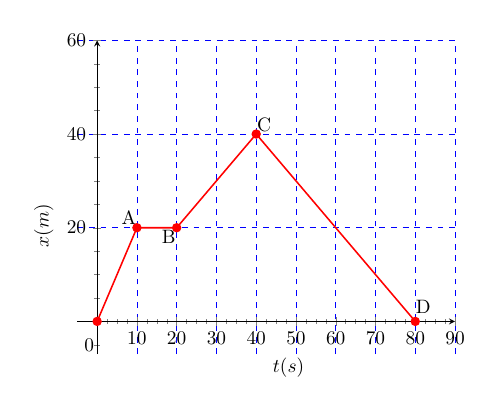
\begin{tikzpicture}[scale=0.7]
                \begin{axis}
                    [axis lines = left,
                    axis x line=center,
                    axis y line=center,
                    xlabel={$t(s)$},
                    ylabel={$x(m)$},
                    ylabel near ticks,
                    xlabel near ticks,
                    xlabel style={below right},
                    ylabel style={above left},
                    ymax=60,
                    ymin=-7,
                    xmax=90,
                    xmin=-5,
                    xtick={0,10,20,30,40,50,60,70,80,90},
                    ymajorgrids=true,
                    xmajorgrids=true,
                    minor tick num=3,
                    grid style={dashed, blue},
                    ]
                    \addplot[red,draw,thick, mark=*, mark options={fill=red}] coordinates {(0,0) (10,20) (20,20) (40,40) (80,0)};
                    \node at (axis cs:8,22) {A};
                    \draw (axis cs:10,20) circle;
                    \node at (axis cs:18,18) {B};
                    \node at (axis cs:42,42) {C};
                    \node at (axis cs:82,3) {D};
                    \node at (axis cs:-2,-5) {0};
                \end{axis}
        \end{tikzpicture}
        \caption{\textbf{Sistema de referencia}. Posición frente a tiempo.}
    \end{figure}
\end{minipage}
% Additional text translation
\vspace*{-6pt}
\begin{itemize}[leftmargin=0pt]
        \item En \( t_B=\qty{20}{\s} \), el ciclista está también en \( x_B = \qty{20}{\metre} \).
        Desde \( t_B=10 \) hasta \( t_C=20 \), el desplazamiento es \qty{0}{\m}, pero el desplazamiento total desde \( x_0 = 0 \) hasta \( x_B = 20 \) es \qty{20}{\m}.
        \item Desde \( x_C = 40 \) hasta \( x_D=0 \), la pendiente de la recta es negativa, lo que indica movimiento hacia atrás.
        El desplazamiento desde \( x_C = 40 \) hasta \( x_D = 0 \) es \qty{40}{\m} hacia atrás.
        Desde \( x_0 = 0 \) hasta \( x_D=80 \), el desplazamiento total es \qty{0}{\m}.
        \item La distancia total recorrida es la suma de cada tramo: \( 20 + 0 + 20 + 40 = \qty{80}{\m} \).
\end{itemize}

\textbf{Análisis del movimiento en cada tramo}:
\begin{itemize}
    \item Tramo 0-A: MRU (línea recta en la gráfica posición-tiempo)
    \item Tramo A-B: Sin movimiento (objeto en reposo)
    \item Tramo B-C: MRU de nuevo
    \item Tramo C-D: MRU hacia atrás
\end{itemize}
Las gráficas muestran la diferencia entre desplazamiento y distancia recorrida.
\section{Gráficas Velocidad-Tiempo}
Las gráficas velocidad-tiempo representan la velocidad de un objeto que se mueve durante un periodo de tiempo determinado.
\begin{figure}[H]
    \centering
    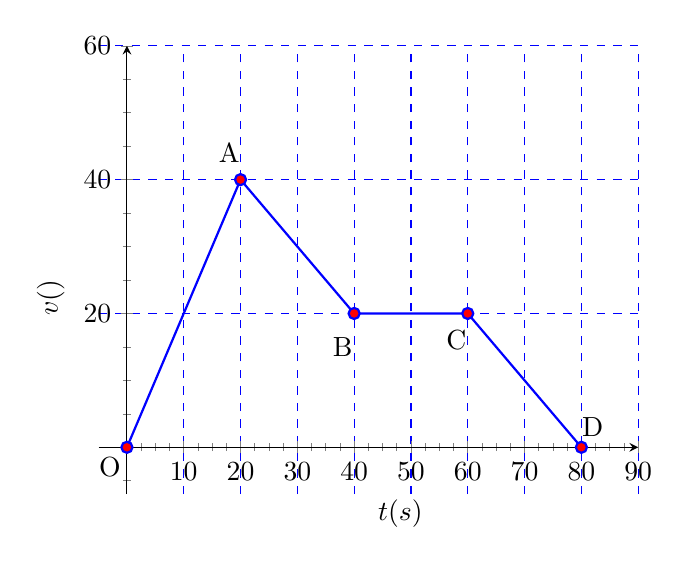
\begin{tikzpicture}[scale=1]
        \centering
        \begin{axis}
            [axis lines = left,
            axis x line=center,
            axis y line=center,
            mark=circle,
            xlabel={$t(s)$},
            ylabel={$v(\unit{\mps})$},
            ylabel near ticks,
            xlabel near ticks,
            xlabel style={below right},
            ylabel style={above left},
            ymax=60,
            ymin=-7,
            xmax=90,
            xmin=-5,
            xtick={0,10,20,30,40,50,60,70,80,90},
            ymajorgrids=true,
            xmajorgrids=true,
            minor tick num=3,
            grid style={dashed, blue},
            ]
            \addplot[blue,draw,thick, mark=*, mark options={fill=red}] coordinates {(0,0) (20,40) (40,20) (60,20) (80,0)};
            \node at (axis cs:18,44) {A};
            \draw (axis cs:10,20) circle;
            \node at (axis cs:38,15) {B};
            \node at (axis cs:58,16) {C};
            \node at (axis cs:82,3) {D};
            \node at (axis cs:-3,-3) {O};
        \end{axis}
    \end{tikzpicture}
    \caption{Gráfica de \( v \) frente a \( t \)}
\end{figure}

\textbf{Análisis del tipo de movimiento en los distintos tramos:}

\begin{itemize}
    \item Tramo O-A: Tenemos un movimiento rectilíneo uniformemente acelerado (MRUA) porque la gráfica velocidad-tiempo es una línea recta, y avanza hacia adelante.
    \item Tramo A-B: También tenemos MRUA, pero ahora moviéndose hacia atrás.
    \item Tramo B-C: Tenemos de nuevo un movimiento rectilíneo uniforme (MRU) porque la velocidad no cambia, por lo que la gráfica es horizontal.
    \item Tramo C-D: Otro MRUA, ahora moviéndose hacia atrás.
\end{itemize}


\begin{exercise}
    La siguiente gráfica muestra el movimiento de un objeto. Responde a las siguientes preguntas:
    \begin{enumerate}[label=\letraminuscula]
    \item ¿Qué tipo de movimiento se produce en cada tramo de la gráfica?
    \item Calcula la aceleración en cada tramo.
    \item ¿Cuál es la distancia total recorrida por el objeto?
    \end{enumerate}

    \begin{figure}[H]
        \centering
        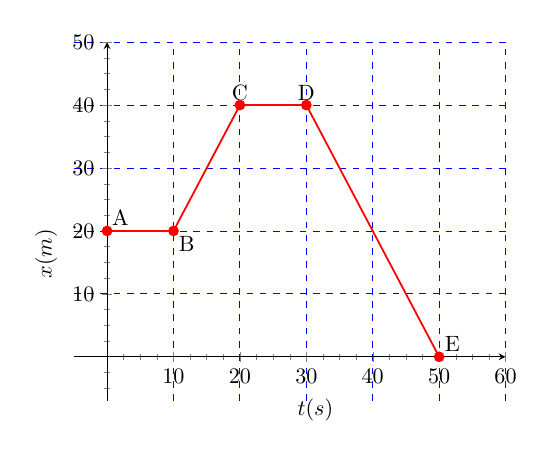
\begin{tikzpicture}[scale=0.8]
                \centering
                \begin{axis}
                    [axis lines = left,
                    axis x line=center,
                    axis y line=center,
                    mark=circle,
                    xlabel={$t(s)$},
                    ylabel={$x(m)$},
                    ylabel near ticks,
                    xlabel near ticks,
                    xlabel style={below right},
                    ylabel style={above left},
                    ymax=50,
                    ymin=-7,
                    xmax=60,
                    xmin=-5,
                    xtick={0,10,20,30,40,50,60},
                    ymajorgrids=true,
                    xmajorgrids=true,
                    minor tick num=3,
                    grid style={dashed, blue},
                    ]
                    \addplot[red,draw,thick, mark=*, mark options={fill=red}] coordinates {(0,20) (10,20) (20,40) (30,40) (50,0)};
                    \node at (axis cs:2,22) {A};
                    \draw (axis cs:10,20) circle;
                    \node at (axis cs:12,18) {B};
                    \node at (axis cs:20,42) {C};
                    \node at (axis cs:30,42) {D};
                    \node at (axis cs:52,2) {E};
                \end{axis}
        \end{tikzpicture}
    \end{figure}

    \begin{solu}
        \textbf{\textcolor{purple}{Ejercicio:}} La siguiente gráfica muestra el movimiento de un objeto. Responde a las siguientes preguntas:
        \begin{enumerate}[label=\letraminuscula]
            \item ¿Qué tipo de movimiento se produce en cada tramo de la gráfica?
            \item Calcula la aceleración en cada tramo.
            \item ¿Cuál es la distancia total recorrida por el objeto?
        \end{enumerate}

        \vspace{0.3cm}

        \textcolor{blue}{Lectura de la gráfica:}
        \begin{itemize}
            \item Punto A: $(0, 20)$ m
            \item Punto B: $(10, 20)$ m
            \item Punto C: $(20, 40)$ m
            \item Punto D: $(30, 40)$ m
            \item Punto E: $(50, 0)$ m
        \end{itemize}

        \textbf{\textcolor{blue}{Apartado a) Tipo de movimiento en cada tramo}}

        \textcolor{blue}{Tramo A-B ($t = 0$ a $t = 10$ s):}
        \begin{itemize}
            \item La posición permanece constante en 20 m
            \item \textcolor{red}{Tipo: En reposo (sin movimiento, $v = 0$)}
        \end{itemize}

        \textcolor{blue}{Tramo B-C ($t = 10$ a $t = 20$ s):}
        \begin{itemize}
            \item La posición aumenta linealmente de 20 m a 40 m
            \item \textcolor{red}{Tipo: Movimiento uniforme (velocidad positiva constante)}
        \end{itemize}

        \textcolor{blue}{Tramo C-D ($t = 20$ a $t = 30$ s):}
        \begin{itemize}
            \item La posición permanece constante en 40 m
            \item \textcolor{red}{Tipo: En reposo (sin movimiento, $v = 0$)}
        \end{itemize}

        \textcolor{blue}{Tramo D-E ($t = 30$ a $t = 50$ s):}
        \begin{itemize}
            \item La posición disminuye linealmente de 40 m a 0 m
            \item \textcolor{red}{Tipo: Movimiento uniforme (velocidad negativa constante - moviéndose hacia atrás)}
        \end{itemize}

        \vspace{0.5cm}

        \textbf{\textcolor{blue}{Apartado b) Calcular la aceleración en cada tramo}}

        \textcolor{red}{Concepto clave:} La aceleración es la tasa de cambio de la velocidad. En las gráficas posición-tiempo, la aceleración está relacionada con la curvatura de la gráfica.

        \textcolor{blue}{Tramo A-B:}
        \[
            v = \frac{\Delta x}{\Delta t} = \frac{20 - 20}{10 - 0} = 0 \text{ m/s}
        \]
        La velocidad es constante (cero), por lo que: $\textcolor{red}{a = 0 \text{ m/s}^2}$

        \textcolor{blue}{Tramo B-C:}
        \[
            v = \frac{\Delta x}{\Delta t} = \frac{40 - 20}{20 - 10} = \frac{20}{10} = 2 \text{ m/s}
        \]
        La velocidad es constante, por lo que: $\textcolor{red}{a = 0 \text{ m/s}^2}$

        \textcolor{blue}{Tramo C-D:}
        \[
            v = \frac{\Delta x}{\Delta t} = \frac{40 - 40}{30 - 20} = 0 \text{ m/s}
        \]
        La velocidad es constante (cero), por lo que: $\textcolor{red}{a = 0 \text{ m/s}^2}$

        \textcolor{blue}{Tramo D-E:}
        \[
            v = \frac{\Delta x}{\Delta t} = \frac{0 - 40}{50 - 30} = \frac{-40}{20} = -2 \text{ m/s}
        \]
        La velocidad es constante, por lo que: $\textcolor{red}{a = 0 \text{ m/s}^2}$

        \textcolor{red}{Resumen:} La aceleración es \textbf{cero} en todos los tramos porque la gráfica está formada por segmentos de línea recta (velocidad constante en cada tramo). La velocidad cambia \textit{instantáneamente} en los puntos B, C y D, lo que requeriría una aceleración infinita, pero esto es una idealización.

        \vspace{0.5cm}

        \textbf{\textcolor{blue}{Apartado c) Distancia total recorrida}}

        \textcolor{red}{Importante:} La distancia es la longitud total del camino recorrido (siempre positiva), independientemente de la dirección.

        \textcolor{blue}{Tramo A-B:}
        \[
            d_{AB} = |20 - 20| = 0 \text{ m}
        \]

        \textcolor{blue}{Tramo B-C:}
        \[
            d_{BC} = |40 - 20| = 20 \text{ m}
        \]

        \textcolor{blue}{Tramo C-D:}
        \[
            d_{CD} = |40 - 40| = 0 \text{ m}
        \]

        \textcolor{blue}{Tramo D-E:}
        \[
            d_{DE} = |0 - 40| = 40 \text{ m}
        \]

        \textcolor{blue}{Distancia total:}
        \[
            d_{\text{total}} = d_{AB} + d_{BC} + d_{CD} + d_{DE}
        \]
        \[
            d_{\text{total}} = 0 + 20 + 0 + 40 = \textcolor{red}{60 \text{ m}}
        \]

        \textcolor{red}{Respuesta c):} La distancia total recorrida por el objeto es \textbf{60 m}.

        \textcolor{blue}{Nota:} El desplazamiento (cambio de posición entre el inicio y el final) sería $0 - 20 = -20$ m, que es diferente de la distancia total recorrida.
    \end{solu}
\end{exercise}

\begin{exercise}
    La siguiente gráfica muestra el movimiento de un objeto. Responde a las siguientes preguntas:
    \begin{enumerate}[label=\letraminuscula]
    \item ¿Qué tipo de movimiento se produce en cada tramo de la gráfica?
    \item Calcula la aceleración en cada tramo.
    \item ¿Cuál es la distancia total recorrida por el objeto?
    \end{enumerate}

    \begin{figure}[H]
        \centering
        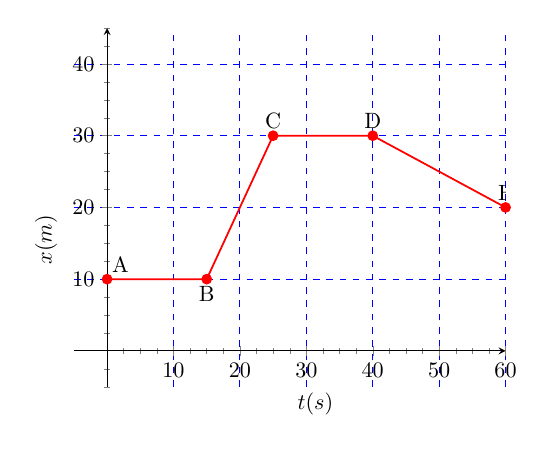
\begin{tikzpicture}[scale=0.8]
                \centering
                \begin{axis}
                    [axis lines = left,
                    axis x line=center,
                    axis y line=center,
                    xlabel={$t(s)$},
                    ylabel={$x(m)$},
                    ylabel near ticks,
                    xlabel near ticks,
                    xlabel style={below right},
                    ylabel style={above left},
                    ymax=45,
                    ymin=-5,
                    xmax=60,
                    xmin=-5,
                    xtick={0,10,20,30,40,50,60},
                    ymajorgrids=true,
                    xmajorgrids=true,
                    minor tick num=3,
                    grid style={dashed, blue},
                    ]
                    \addplot[red,draw,thick, mark=*, mark options={fill=red}] coordinates {(0,10) (15,10) (25,30) (40,30) (60,20)};
                    \node at (axis cs:2,12) {A};
                    \node at (axis cs:15,8) {B};
                    \node at (axis cs:25,32) {C};
                    \node at (axis cs:40,32) {D};
                    \node at (axis cs:60,22) {E};
                \end{axis}
        \end{tikzpicture}
    \end{figure}

    \begin{solu}
        \textbf{\textcolor{purple}{Ejercicio:}} La siguiente gráfica muestra el movimiento de un objeto. Responde a las siguientes preguntas:
        \begin{enumerate}[label=\letraminuscula]
            \item ¿Qué tipo de movimiento se produce en cada tramo de la gráfica?
            \item Calcula la aceleración en cada tramo.
            \item ¿Cuál es la distancia total recorrida por el objeto?
        \end{enumerate}

        \vspace{0.3cm}

        \textcolor{blue}{Lectura de la gráfica:}
        \begin{itemize}
            \item Punto A: $(0,10)$ m
            \item Punto B: $(15,10)$ m
            \item Punto C: $(25,30)$ m
            \item Punto D: $(40,30)$ m
            \item Punto E: $(60,20)$ m
        \end{itemize}

        \textbf{\textcolor{blue}{Apartado a) Tipo de movimiento en cada tramo}}

        \textcolor{blue}{Tramo A-B ($t=0$ a $15$ s):}
        \begin{itemize}
            \item La posición permanece constante.
            \item \textcolor{red}{Tipo: En reposo ($v=0$).}
        \end{itemize}

        \textcolor{blue}{Tramo B-C ($t=15$ a $25$ s):}
        \begin{itemize}
            \item La posición aumenta linealmente.
            \item \textcolor{red}{Tipo: Movimiento uniforme (velocidad positiva constante).}
        \end{itemize}

        \textcolor{blue}{Tramo C-D ($t=25$ a $40$ s):}
        \begin{itemize}
            \item La posición permanece constante.
            \item \textcolor{red}{Tipo: En reposo ($v=0$).}
        \end{itemize}

        \textcolor{blue}{Tramo D-E ($t=40$ a $60$ s):}
        \begin{itemize}
            \item La posición disminuye linealmente.
            \item \textcolor{red}{Tipo: Movimiento uniforme (velocidad negativa constante).}
        \end{itemize}

        \vspace{0.5cm}

        \textbf{\textcolor{blue}{Apartado b) Calcular la aceleración en cada tramo}}

        \textcolor{blue}{Tramo A-B:}
        \[
        v=\frac{10-10}{15-0}=0\text{ m/s}
        \]
        Por lo tanto,
        \[
        \boxed{a=0\text{ m/s}^2}
        \]

        \textcolor{blue}{Tramo B-C:}
        \[
        v=\frac{30-10}{25-15}=\frac{20}{10}=2\text{ m/s}
        \]
        Por lo tanto,
        \[
        \boxed{a=0\text{ m/s}^2}
        \]

        \textcolor{blue}{Tramo C-D:}
        \[
        v=\frac{30-30}{40-25}=0\text{ m/s}
        \]
        Por lo tanto,
        \[
        \boxed{a=0\text{ m/s}^2}
        \]

        \textcolor{blue}{Tramo D-E:}
        \[
        v=\frac{20-30}{60-40}=\frac{-10}{20}=-0.5\text{ m/s}
        \]
        Por lo tanto,
        \[
        \boxed{a=0\text{ m/s}^2}
        \]

        \textcolor{red}{La aceleración es cero en todos los tramos porque la velocidad es constante en cada intervalo.}

        \vspace{0.5cm}

        \textbf{\textcolor{blue}{Apartado c) Distancia total recorrida}}

        \[
        d_{AB}=0\text{ m}
        \]

        \[
        d_{BC}=20\text{ m}
        \]

        \[
        d_{CD}=0\text{ m}
        \]

        \[
        d_{DE}=10\text{ m}
        \]

        \[
        d_{\text{total}}=0+20+0+10=\boxed{30\text{ m}}
        \]

        \textcolor{blue}{El desplazamiento es $20-10=10$ m.}
    \end{solu}
\end{exercise}

\begin{exercise}
    La siguiente gráfica muestra el movimiento de un objeto. Responde a las siguientes preguntas:
    \begin{enumerate}[label=\letraminuscula]
    \item ¿Qué tipo de movimiento se produce en cada tramo de la gráfica?
    \item Calcula la aceleración en cada tramo.
    \item ¿Cuál es la distancia total recorrida por el objeto?
    \end{enumerate}

    \begin{figure}[H]
        \centering
        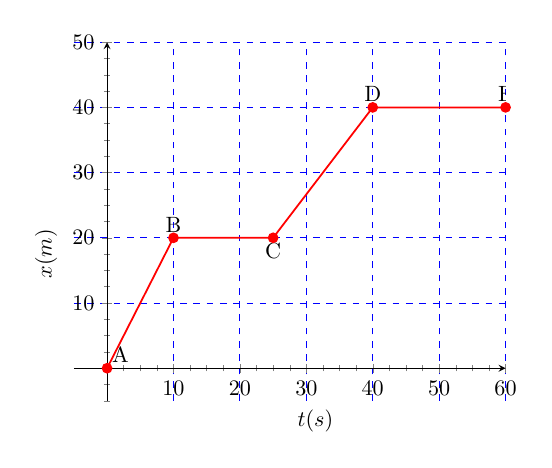
\begin{tikzpicture}[scale=0.8]
                \centering
                \begin{axis}
                    [axis lines = left,
                    axis x line=center,
                    axis y line=center,
                    xlabel={$t(s)$},
                    ylabel={$x(m)$},
                    ylabel near ticks,
                    xlabel near ticks,
                    xlabel style={below right},
                    ylabel style={above left},
                    ymax=50,
                    ymin=-5,
                    xmax=60,
                    xmin=-5,
                    xtick={0,10,20,30,40,50,60},
                    ymajorgrids=true,
                    xmajorgrids=true,
                    minor tick num=3,
                    grid style={dashed, blue},
                    ]
                    \addplot[red,draw,thick, mark=*, mark options={fill=red}] coordinates {(0,0) (10,20) (25,20) (40,40) (60,40)};
                    \node at (axis cs:2,2) {A};
                    \node at (axis cs:10,22) {B};
                    \node at (axis cs:25,18) {C};
                    \node at (axis cs:40,42) {D};
                    \node at (axis cs:60,42) {E};
                \end{axis}
        \end{tikzpicture}
    \end{figure}

    \begin{solu}
        \textbf{\textcolor{purple}{Ejercicio:}} La siguiente gráfica muestra el movimiento de un objeto. Responde a las siguientes preguntas:
        \begin{enumerate}[label=\letraminuscula]
            \item ¿Qué tipo de movimiento se produce en cada tramo de la gráfica?
            \item Calcula la aceleración en cada tramo.
            \item ¿Cuál es la distancia total recorrida por el objeto?
        \end{enumerate}

        \vspace{0.3cm}

        \textcolor{blue}{Lectura de la gráfica:}
        \begin{itemize}
            \item Punto A: $(0,0)$ m
            \item Punto B: $(10,20)$ m
            \item Punto C: $(25,20)$ m
            \item Punto D: $(40,40)$ m
            \item Punto E: $(60,40)$ m
        \end{itemize}

        \textbf{\textcolor{blue}{Apartado a) Tipo de movimiento en cada tramo}}

        \textcolor{blue}{Tramo A-B:}
        \begin{itemize}
            \item La posición aumenta linealmente.
            \item \textcolor{red}{Tipo: Movimiento uniforme (velocidad positiva constante).}
        \end{itemize}

        \textcolor{blue}{Tramo B-C:}
        \begin{itemize}
            \item La posición permanece constante.
            \item \textcolor{red}{Tipo: En reposo.}
        \end{itemize}

        \textcolor{blue}{Tramo C-D:}
        \begin{itemize}
            \item La posición aumenta linealmente.
            \item \textcolor{red}{Tipo: Movimiento uniforme (velocidad positiva constante).}
        \end{itemize}

        \textcolor{blue}{Tramo D-E:}
        \begin{itemize}
            \item La posición permanece constante.
            \item \textcolor{red}{Tipo: En reposo.}
        \end{itemize}

        \vspace{0.5cm}

        \textbf{\textcolor{blue}{Apartado b) Calcular la aceleración en cada tramo}}

        \textcolor{blue}{Tramo A-B:}
        \[
        v=\frac{20-0}{10-0}=2\text{ m/s}
        \]
        Por lo tanto,
        \[
        \boxed{a=0\text{ m/s}^2}
        \]

        \textcolor{blue}{Tramo B-C:}
        \[
        v=\frac{20-20}{25-10}=0\text{ m/s}
        \]
        Por lo tanto,
        \[
        \boxed{a=0\text{ m/s}^2}
        \]

        \textcolor{blue}{Tramo C-D:}
        \[
        v=\frac{40-20}{40-25}=\frac{20}{15}=1.33\text{ m/s}
        \]
        Por lo tanto,
        \[
        \boxed{a=0\text{ m/s}^2}
        \]

        \textcolor{blue}{Tramo D-E:}
        \[
        v=\frac{40-40}{60-40}=0\text{ m/s}
        \]
        Por lo tanto,
        \[
        \boxed{a=0\text{ m/s}^2}
        \]

        \textcolor{red}{La aceleración es cero en todos los tramos porque cada segmento es una línea recta.}

        \vspace{0.5cm}

        \textbf{\textcolor{blue}{Apartado c) Distancia total recorrida}}

        \[
        d_{AB}=20\text{ m}
        \]

        \[
        d_{BC}=0\text{ m}
        \]

        \[
        d_{CD}=20\text{ m}
        \]

        \[
        d_{DE}=0\text{ m}
        \]

        \[
        d_{\text{total}}=20+0+20+0=\boxed{40\text{ m}}
        \]

        \textcolor{blue}{El desplazamiento es $40-0=40$ m.}
    \end{solu}
\end{exercise}

\begin{exercise}
    La siguiente gráfica muestra la velocidad de un objeto. Responde a las siguientes preguntas:
    \begin{enumerate}[label=\letraminuscula]
    \item ¿Qué tipo de movimiento se produce en cada tramo de la gráfica?
    \item Calcula la aceleración en cada tramo.
    \item ¿Cuál es la distancia total recorrida por el objeto?
    \end{enumerate}

    \begin{figure}[H]
        \centering
        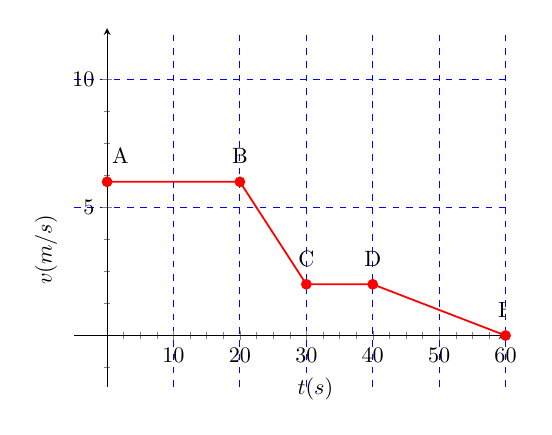
\begin{tikzpicture}[scale=0.8]
            \begin{axis}
                [axis lines = left,
                axis x line=center,
                axis y line=center,
                xlabel={$t(s)$},
                ylabel={$v(m/s)$},
                ylabel near ticks,
                xlabel near ticks,
                xlabel style={below right},
                ylabel style={above left},
                ymax=12,
                ymin=-2,
                xmax=60,
                xmin=-5,
                xtick={0,10,20,30,40,50,60},
                ymajorgrids=true,
                xmajorgrids=true,
                minor tick num=3,
                grid style={dashed, blue},
                ]
                \addplot[red,draw,thick,mark=*,mark options={fill=red}]
                coordinates {(0,6) (20,6) (30,2) (40,2) (60,0)};
                \node at (axis cs:2,7) {A};
                \node at (axis cs:20,7) {B};
                \node at (axis cs:30,3) {C};
                \node at (axis cs:40,3) {D};
                \node at (axis cs:60,1) {E};
            \end{axis}
        \end{tikzpicture}
    \end{figure}

    \begin{solu}

    \textbf{\textcolor{purple}{Ejercicio:}} La siguiente gráfica muestra la velocidad de un objeto.

    \textcolor{blue}{Lectura de la gráfica:}
    \begin{itemize}
        \item A: $(0,6)$ m/s
        \item B: $(20,6)$ m/s
        \item C: $(30,2)$ m/s
        \item D: $(40,2)$ m/s
        \item E: $(60,0)$ m/s
    \end{itemize}

    \textbf{\textcolor{blue}{Apartado a) Tipo de movimiento}}

    \textbf{A-B:}
    \begin{itemize}
        \item Velocidad constante.
        \item \textcolor{red}{Movimiento uniforme.}
    \end{itemize}

    \textbf{B-C:}
    \begin{itemize}
        \item La velocidad disminuye de manera uniforme.
        \item \textcolor{red}{Movimiento uniformemente decelerado.}
    \end{itemize}

    \textbf{C-D:}
    \begin{itemize}
        \item Velocidad constante.
        \item \textcolor{red}{Movimiento uniforme.}
    \end{itemize}

    \textbf{D-E:}
    \begin{itemize}
        \item La velocidad disminuye de manera uniforme.
        \item \textcolor{red}{Movimiento uniformemente decelerado.}
    \end{itemize}

    \textbf{\textcolor{blue}{Apartado b) Aceleración}}

    A-B:
    \[
    a=\frac{6-6}{20}=0\text{ m/s}^2
    \]

    B-C:
    \[
    a=\frac{2-6}{10}=-0.4\text{ m/s}^2
    \]

    C-D:
    \[
    a=\frac{2-2}{10}=0\text{ m/s}^2
    \]

    D-E:
    \[
    a=\frac{0-2}{20}=-0.1\text{ m/s}^2
    \]

    \textbf{\textcolor{blue}{Apartado c) Distancia total}}

    Área A-B:
    \[
    (20)(6)=120\text{ m}
    \]

    Área B-C:
    \[
    \frac{6+2}{2}(10)=40\text{ m}
    \]

    Área C-D:
    \[
    (10)(2)=20\text{ m}
    \]

    Área D-E:
    \[
    \frac{2+0}{2}(20)=20\text{ m}
    \]

    Distancia total:
    \[
    d=120+40+20+20=\boxed{200\text{ m}}
    \]

    \end{solu}
\end{exercise}

\begin{exercise}
    La siguiente gráfica muestra la velocidad de un objeto. Responde a las siguientes preguntas:
    \begin{enumerate}[label=\letraminuscula]
    \item ¿Qué tipo de movimiento se produce en cada tramo de la gráfica?
    \item Calcula la aceleración en cada tramo.
    \item ¿Cuál es la distancia total recorrida por el objeto?
    \end{enumerate}

    \begin{figure}[H]
        \centering
        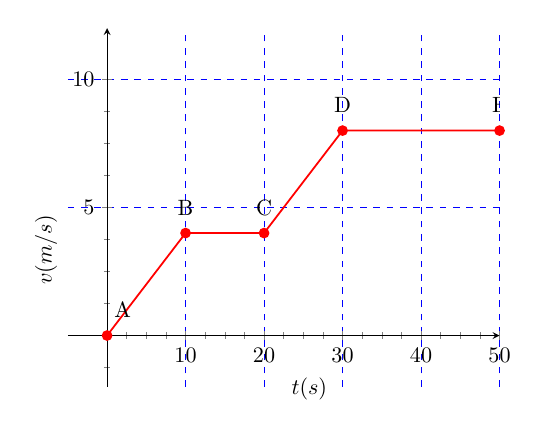
\begin{tikzpicture}[scale=0.8]
            \begin{axis}
                [axis lines = left,
                axis x line=center,
                axis y line=center,
                xlabel={$t(s)$},
                ylabel={$v(m/s)$},
                ylabel near ticks,
                xlabel near ticks,
                xlabel style={below right},
                ylabel style={above left},
                ymax=12,
                ymin=-2,
                xmax=50,
                xmin=-5,
                xtick={0,10,20,30,40,50},
                ymajorgrids=true,
                xmajorgrids=true,
                minor tick num=3,
                grid style={dashed, blue},
                ]
                \addplot[red,draw,thick,mark=*,mark options={fill=red}]
                coordinates {(0,0) (10,4) (20,4) (30,8) (50,8)};
                \node at (axis cs:2,1) {A};
                \node at (axis cs:10,5) {B};
                \node at (axis cs:20,5) {C};
                \node at (axis cs:30,9) {D};
                \node at (axis cs:50,9) {E};
            \end{axis}
        \end{tikzpicture}
    \end{figure}

    \begin{solu}

    \textbf{\textcolor{purple}{Ejercicio:}} La siguiente gráfica muestra la velocidad de un objeto.

    \textcolor{blue}{Lectura de la gráfica:}
    \begin{itemize}
        \item A: $(0,0)$ m/s
        \item B: $(10,4)$ m/s
        \item C: $(20,4)$ m/s
        \item D: $(30,8)$ m/s
        \item E: $(50,8)$ m/s
    \end{itemize}

    \textbf{\textcolor{blue}{Apartado a) Tipo de movimiento}}

    \textbf{A-B:}
    \begin{itemize}
        \item La velocidad aumenta de manera uniforme.
        \item \textcolor{red}{Movimiento uniformemente acelerado.}
    \end{itemize}

    \textbf{B-C:}
    \begin{itemize}
        \item Velocidad constante.
        \item \textcolor{red}{Movimiento uniforme.}
    \end{itemize}

    \textbf{C-D:}
    \begin{itemize}
        \item La velocidad aumenta de manera uniforme.
        \item \textcolor{red}{Movimiento uniformemente acelerado.}
    \end{itemize}

    \textbf{D-E:}
    \begin{itemize}
        \item Velocidad constante.
        \item \textcolor{red}{Movimiento uniforme.}
    \end{itemize}

    \textbf{\textcolor{blue}{Apartado b) Aceleración}}

    A-B:
    \[
    a=\frac{4-0}{10}=0.4\text{ m/s}^2
    \]

    B-C:
    \[
    a=\frac{4-4}{10}=0\text{ m/s}^2
    \]

    C-D:
    \[
    a=\frac{8-4}{10}=0.4\text{ m/s}^2
    \]

    D-E:
    \[
    a=\frac{8-8}{20}=0\text{ m/s}^2
    \]

    \textbf{\textcolor{blue}{Apartado c) Distancia total}}

    Área A-B:
    \[
    \frac12(10)(4)=20\text{ m}
    \]

    Área B-C:
    \[
    (10)(4)=40\text{ m}
    \]

    Área C-D:
    \[
    \frac{4+8}{2}(10)=60\text{ m}
    \]

    Área D-E:
    \[
    (20)(8)=160\text{ m}
    \]

    Distancia total:
    \[
    d=20+40+60+160=\boxed{280\text{ m}}
    \]

    \end{solu}
\end{exercise}

\begin{exercise}
    Elabora un mapa conceptual que resuma los principales temas de esta unidad.
    \begin{solu}
        \textbf{\textcolor{purple}{Ejercicio:}} Elabora un mapa conceptual que resuma los principales temas de esta unidad.

        \textcolor{blue}{Este es un ejercicio abierto en el que el alumnado debe crear su propio mapa conceptual incluyendo términos clave como: posición, desplazamiento, velocidad, rapidez, aceleración, movimiento uniforme, movimiento uniformemente acelerado, gráficas posición-tiempo, gráficas velocidad-tiempo, ecuaciones cinemáticas, etc.}
    \end{solu}
\end{exercise}

%\section{Vocabulary}
%
%\begin{vocabulary}[Kinematics]
%The branch of Physics that studies motion without taking into account the causes that produce it. It focuses on describing how objects move through space and time. \newline
%\textbf{Translation to Spanish}: Cinemática \newline
%% Line 9
%\end{vocabulary}
%
%\begin{vocabulary}[Motion]
%The change in position of an object with respect to a reference system over time. An object is in motion when its position changes relative to a chosen reference point. \newline
%\textbf{Translation to Spanish}: Movimiento \newline
%% Line 49
%\end{vocabulary}
%
%\begin{vocabulary}[Rest]
%The state of an object when its position does not change with respect to a reference system over time. \newline
%\textbf{Translation to Spanish}: Reposo \newline
%% Line 51
%\end{vocabulary}
%
%\begin{vocabulary}[Reference System]
%A system that allows us to fix the position of an object and study its evolution over time. In Physics, it is usually a Cartesian coordinate system (x, y). \newline
%\textbf{Translation to Spanish}: Sistema de referencia \newline
%% Line 58
%\end{vocabulary}
%
%\begin{vocabulary}[Position]
%The exact location of an object in space, usually represented by the letter x. The SI unit is the meter (m). \newline
%\textbf{Translation to Spanish}: Posición \newline
%% Line 69
%\end{vocabulary}
%
%\begin{vocabulary}[Displacement]
%The difference between the final position and the initial position of the motion, represented as \( \Delta x = x_f - x_i \). It is a vector quantity that can be positive or negative. The SI unit is the meter (m). \newline
%\textbf{Translation to Spanish}: Desplazamiento \newline
%% Line 73
%\end{vocabulary}
%
%\begin{vocabulary}[Trajectory]
%The path followed by an object during its motion. It can be rectilinear (straight line), circular, or curvilinear (curved). \newline
%\textbf{Translation to Spanish}: Trayectoria \newline
%% Line 103
%\end{vocabulary}
%
%\begin{vocabulary}[Distance Travelled]
%The length of the trajectory followed by an object. It is a scalar quantity always positive. The SI unit is the meter (m). \newline
%\textbf{Translation to Spanish}: Distancia recorrida \newline
%% Line 106
%\end{vocabulary}
%
%\begin{vocabulary}[Rectilinear Motion]
%Motion in which the trajectory is a straight line. In this type of motion, displacement coincides with the distance traveled. \newline
%\textbf{Translation to Spanish}: Movimiento rectilíneo \newline
%% Line 114
%\end{vocabulary}
%
%\begin{vocabulary}[Circular Motion]
%Motion in which the trajectory is circular or describes a circle. \newline
%\textbf{Translation to Spanish}: Movimiento circular \newline
%% Line 117
%\end{vocabulary}
%
%\begin{vocabulary}[Curvilinear Motion]
%Motion in which the trajectory describes curves that are neither straight lines nor perfect circles. \newline
%\textbf{Translation to Spanish}: Movimiento curvilíneo \newline
%% Line 119
%\end{vocabulary}
%
%\begin{vocabulary}[Velocity]
%The rate of change of position with respect to time. It is a vector quantity that indicates both speed and direction. The SI unit is meters per second (m/s). \newline
%\textbf{Translation to Spanish}: Velocidad \newline
%% Line 201 (approximately, appears throughout the document)
%\end{vocabulary}
%
%\begin{vocabulary}[Speed]
%The magnitude of velocity, representing how fast an object is moving without regard to direction. It is a scalar quantity. The SI unit is meters per second (m/s). \newline
%\textbf{Translation to Spanish}: Rapidez \newline
%% Line 201 (approximately, appears throughout the document)
%\end{vocabulary}
%
%\begin{vocabulary}[Average Velocity]
%The total displacement divided by the total time taken. It is calculated as \( v_{avg} = \Delta x / \Delta t \) \newline
%\textbf{Translation to Spanish}: Velocidad media \newline
%% Line 201 (approximately, appears in context)
%\end{vocabulary}
%
%\begin{vocabulary}[Instantaneous Velocity]
%The velocity of an object at a specific instant of time. It is the limit of average velocity as the time interval approaches zero. \newline
%\textbf{Translation to Spanish}: Velocidad instantánea \newline
%% Line 201 (approximately, appears in context)
%\end{vocabulary}
%
%\begin{vocabulary}[Acceleration]
%The rate of change of velocity with respect to time. It is a vector quantity. The SI unit is meters per second squared (m/s²). \newline
%\textbf{Translation to Spanish}: Aceleración \newline
%% Line 201 (approximately, appears throughout the document)
%\end{vocabulary}
%
%\begin{vocabulary}[Uniform Rectilinear Motion (URM)]
%Motion in a straight line with constant velocity (zero acceleration). The object covers equal distances in equal time intervals. \newline
%\textbf{Translation to Spanish}: Movimiento rectilíneo uniforme (MRU) \newline
%% Line 2346
%\end{vocabulary}
%
%\begin{vocabulary}[Uniformly Accelerated Rectilinear Motion (UARM)]
%Motion in a straight line with constant acceleration. The velocity changes uniformly over time. Also known as uniformly varied motion. \newline
%\textbf{Translation to Spanish}: Movimiento rectilíneo uniformemente acelerado (MRUA) \newline
%% Line 2399
%\end{vocabulary}
%
%\begin{vocabulary}[Coordinate System]
%A system used to specify the position of a point in space using numerical coordinates. The most common is the Cartesian coordinate system. \newline
%\textbf{Translation to Spanish}: Sistema de coordenadas \newline
%% Line 55
%\end{vocabulary}
%
%\begin{vocabulary}[Origin]
%The reference point in a coordinate system where all coordinates are zero. It serves as the starting point for measuring position. \newline
%\textbf{Translation to Spanish}: Origen \newline
%% Line 2288
%\end{vocabulary}
%
%\begin{vocabulary}[Time Interval]
%The difference between two moments in time, calculated as \( \Delta t = t_f - t_i \). It represents the duration of an event or motion. \newline
%\textbf{Translation to Spanish}: Intervalo de tiempo \newline
%% Line 94
%\end{vocabulary}
%
%\begin{vocabulary}[Position-Time Graph]
%A graphical representation showing how an object's position changes over time. The slope of the graph represents velocity. \newline
%\textbf{Translation to Spanish}: Gráfica posición-tiempo \newline
%% Line 2283
%\end{vocabulary}
%
%\begin{vocabulary}[Velocity-Time Graph]
%A graphical representation showing how an object's velocity changes over time. The slope represents acceleration, and the area under the curve represents displacement. \newline
%\textbf{Translation to Spanish}: Gráfica velocidad-tiempo \newline
%% Line 2355
%\end{vocabulary}
%
%\begin{vocabulary}[Slope]
%In a graph, the slope represents the rate of change of the vertical quantity with respect to the horizontal quantity. In position-time graphs, slope represents velocity; in velocity-time graphs, it represents acceleration. \newline
%\textbf{Translation to Spanish}: Pendiente \newline
%% Line 2337
%\end{vocabulary}
%
%\begin{vocabulary}[Vector Quantity]
%A physical quantity that has both magnitude and direction. Examples include displacement, velocity, and acceleration. \newline
%\textbf{Translation to Spanish}: Magnitud vectorial \newline
%% Line 159
%\end{vocabulary}
%
%\begin{vocabulary}[Scalar Quantity]
%A physical quantity that has only magnitude but no direction. Examples include distance, speed, and time. \newline
%\textbf{Translation to Spanish}: Magnitud escalar \newline
%% Line 107 (implied in context)
%\end{vocabulary}
%
%\begin{vocabulary}[Initial Position]
%The position of an object at the beginning of motion or at the start of observation, represented as \( x_i \) or \(v  \). \newline
%\textbf{Translation to Spanish}: Posición inicial \newline
%% Line 83
%\end{vocabulary}
%
%\begin{vocabulary}[Final Position]
%The position of an object at the end of motion or at a specific moment, represented as \( x_f \) . \newline
%\textbf{Translation to Spanish}: Posición final \newline
%% Line 81
%\end{vocabulary}
%
%\begin{vocabulary}[Cartesian Coordinate System]
%A coordinate system that uses perpendicular axes (typically x and y in 2D, or x, y, and z in 3D) to specify positions in space. \newline
%\textbf{Translation to Spanish}: Sistema de coordenadas cartesianas \newline
%% Line 55
%\end{vocabulary}
%
%\begin{vocabulary}[Frame of Reference]
%A perspective from which motion is observed and measured. Motion is relative and depends on the chosen frame of reference. \newline
%\textbf{Translation to Spanish}: Sistema de referencia \newline
%% Line 53
%\end{vocabulary}
%
%
%%\begin{exercise}
%%    Vocabulary
%%
%%    \begin{multicols}{2}
%%        \begin{enumerate}
%%            \item Acceleration
%%            \item at rest
%%            \item Average
%%            \item Axis
%%            \item Coordinate System
%%            \item Deform
%%            \item Direction
%%            \item displacement
%%            \item Frame of reference
%%            \item Instantaneous
%%            \item Interval
%%            \item Law
%%            \item Motion
%%            \item Origin
%%            \item Slope
%%            \item Speed
%%            \item Trajectory
%%            \item Uniform rectilinear motion.
%%        \end{enumerate}
%%    \end{multicols}
%
%%\end{exercise}
%
%
%
%
%
%
